\documentclass[a4paper,12pt]{article}
\usepackage{caption}
\usepackage{caption}
\usepackage[utf8]{inputenc}
\usepackage[bottom,hang]{footmisc}
\usepackage[german]{babel}
\usepackage{nameref}
\usepackage[table,xcdraw]{xcolor}
\usepackage{graphicx}
\usepackage{svg}	
\usepackage{listings}
\usepackage{url}
\usepackage{xcolor}
\usepackage{textcomp}
\usepackage{graphicx}
\usepackage{wrapfig}
\usepackage{german}
\usepackage{fancyhdr}
\usepackage{comment}
\usepackage[onehalfspacing]{setspace}
\bibliographystyle{ieeetr}
\usepackage[left=4cm,right=2cm,top=4cm,bottom=2cm,includefoot]{geometry}
\sloppy
\graphicspath{{images/}}

\captionsetup[table]{position=bottom}
\lstset { %
    language=C++,
    backgroundcolor=\color{black!5}, % set backgroundcolor
    basicstyle=\footnotesize,% basic font setting
}


\DeclareCaptionType{code}[Quellcode][Quellcodeverzeichnis] 


\begin{document}
\begin{titlepage}
	\centering
	
\includegraphics[width=0.3\textwidth]{logo}\par\vspace{1cm}
	{\scshape\LARGE Hochschule für Angewandte Wissenschaften Hof \par}
	\vspace{1cm}
	{\scshape\Large Seminararbeit\par}
	\vspace{1.5cm}
	{\huge\bfseries Aufbau und Funktionsweise eines Prozessors\par}
	\vspace{2cm}
	{\Large\itshape Marco Vogel\par}
	\vfill
	unter Aufsicht von\par
	\Large Stefan Müller
	\vfill
% Bottom of the page
	{\large\today\par}
\end{titlepage}
\newpage

\pagestyle{empty} 
\tableofcontents
\newpage
\pagestyle{fancy}
\fancyhf{}
\fancyhead[L]{\rightmark}
\fancyhead[R]{\thepage}
\renewcommand{\headrulewidth}{1pt}
\setlength{\footnotemargin}{0pt}
\setcounter{page}{1}

\section{Motivation}
Die vorliegende Arbeit soll die Faszination der technischen Entwicklung und der Möglichkeiten von Prozessoren aufzeigen. Äußerst interessant ist für mich der stetige Fortschritt der Prozessorentwicklung. Wir nutzen Prozessoren täglich und dennoch ist wenig über die Komplexität dieses Themas bekannt.

\section{Zahlensysteme}

\subsection{Allgemeines}
Das für Menschen geläufige Zahlensystem ist das Dezimalsystem. Das bedeutet, dass Zahlen mit folgender Formel gebildet werden:
$$Z=\sum\limits_{i=0}^{n-1} a_i * 10^i \ \cite[S.11]{mikroprozessortechnik2011}$$
Die Dezimalzahl 135 wird mit dieser Formel wie folgt gebildet:$$Z=1*10^2+3*10^1+5*10^0 = 135$$
Die Basis der Wertepotenz spiegelt das Zahlensystem wieder, welches dargestellt wird. Deshalb ist die Formel für die Zahl $Z$ mit Basis $B$ im Allgemeinen darstellbar als
$$Z=\sum\limits_{i=0}^{n-1} a_i * B^i \ \cite[S.11]{mikroprozessortechnik2011}$$ 
Das dezimale Zahlensystem ist für Menschen sehr intuitiv zu verstehen. Da wir zehn Finger haben, können wir optimal mit der Basis 10 zählen. Für Computer ist dieses Zahlensystem allerdings ungeeignet. Ein Prozessor besteht aus vielen kleinen Transistoren. Diese können entweder Strom fließen lassen oder nicht. Somit bietet sich ein Zahlensystem an, welches nur zwei Zustände kennt: AN und AUS. Strom kann fliesen oder Strom kann nicht fliesen. Der deutsche Mathematiker Gottfried Wilhelm Leibniz (1646-1716) entwickelte die Dyadik; die Darstellung von Zahlen durch 1 und 0. Diese Darstellungsform ist für Prozessoren optimal geeignet, da diese selbst ebenfalls nur zwei Zustände kennen.\cite{mikroprozessortechnik2011}.

\subsection{Binäre Darstellung von Zahlen}

\subsubsection{Vorzeichenlose Binärzahlen}
Vorzeichenlose Binärzahlen können mittels folgender Formel gebildet werden: $$Z=\sum\limits_{i=0}^{N-1} a_i * 2^i$$ 
Die Dezimalzahl 135 würde dann im Dualsystem dem Bitmuster $10000111$ entsprechen; dargestellt durch folgende Konvertierung:
$$10000111b = 1*2^7+0*2^6+0*2^5+0*2^4+0*2^3+1*2^2+1*2^1+1*2^0 = 128 +4+2+1 = 135d$$
Prozessoren haben immer eine begrenzte Anzahl an Bits zur Verfügung, mit welchen sie arbeiten können. In den Anfängen der Prozessorentwicklung waren 8 bzw. 16 Bit Prozessoren üblich. Durch diese Limitation der Bitbreite können ungewollte Probleme beim Rechnen mit Dualzahlen auftreten. So kann es während der Ausführung mit vorzeichenlosen Zahlen zu einem Übertrag kommen. Ein Übertrag tritt auf, wenn zum Beispiel auf einer 8-Bit CPU\footnote{CPU =  Central Processing Unit = Prozessor} die Operation 255+1 ausgeführt wird.

\begin{table}[!htb]
\centering
\begin{tabular}{|c|r|r|}
\hline
\textbf{Übertrag}               & \multicolumn{1}{c|}{\textbf{Binär}} & \multicolumn{1}{c|}{\textbf{Dezimal}} \\ \hline
-                               & 11111111b                            & 255d                                   \\ \hline
-                               & 00000001b                            & +1d                                     \\ \hline
\multicolumn{1}{|r|}{1}         & 00000000b                            & 256d                                   \\ \hline\hline
\multicolumn{1}{|r|}{Ergebnis:} & 00000000b                            & 0d                                     \\ \hline
\end{tabular}
\caption{Rechnung mit Übertrag}
\centering
\small Quelle: Eigene Darstellung
\label{tab:uebertrag}
\end{table}

\noindent In Tabelle \ref{tab:uebertrag} ist diese Rechnung zur Veranschaulichung abgebildet. Aufgrund der Bitbreite des Prozessors von 8-Bit ist die größte darstellbare Binärzahl, welche dieser verarbeiten kann, dargestellt durch acht Einsen ($11111111b = 255d$)\footnote{Die Buchstaben am Ende der Zahlen zeigen das benutzte Zahlensystem. D.h. d = Dezimal, b = Binär, h = Hexadezimal}. \mbox{Nun wird allerdings in Tabelle \ref{tab:uebertrag} diese Zahl inkrementiert\footnote{inkrementiert = um eins erhöht}. }Der Prozessor wird am Ende dieser Operation den Wert null als Ergebnis speichern. Der Grund dafür ist in der letzten Zeile der Tabelle \ref{tab:uebertrag} ersichtlich. Die Rechenoperation 255+1d ergibt 256. Diese Zahl wird im Binärsystem mit 9-Bit dargestellt.
$$256d = 1*2^8+0*2^7+0*2^6+0*2^5+0*2^4+0*2^3+0*2^2+0*2^1+0*2^0 = 100000000b$$
Der Prozessor speichert nur 8 Bit als Ergebnis. Deshalb werden die ersten 8 Bit des Ergebnisses ($00000000b$) gespeichert und die Rechnung ist fehlerhaft. Diese Rechenoperation würde in der CPU das Carry Flag (Übertragsbit) setzen, um dem Entwickler darauf hinzuweisen, dass die letzte Operation ein falsches Ergebnis geliefert hat. 
\subsubsection{Vorzeichenbehaftete Binärzahlen}
\noindent Mit vorzeichenlosen Dualzahlen können allerdings keine negativen Werte abgebildet werden. Diese Eigenschaft bieten vorzeichenbehaftete Dualzahlen. Eine Dualzahl $Z$ im sogenannten Zweierkomplement wird folgendermaßen gebildet:
$$Z=-a_{N-1}*2^{N-1}+\sum\limits_{i=0}^{N-2} a_i * 2^i$$
Die Formel kann zu Erklärungszwecken in zwei Teile gegliedert werden. Zum einen in den ersten Teil $-a_{N-1}*2^{N-1}$, das Vorzeichenbit. Dieser sagt aus, dass das höchstwertige Bit einer vorzeichenbehafteten Zahl negativ gewertet wird. Zum anderen der hintere Teil $\sum\limits_{i=0}^{N-2} a_i * 2^i$, dieser ist bereits aus der Erzeugung von vorzeichenlosen Dualzahlen bekannt. Die Bits werden nach ihrer Position gewichtet und ihre Wertigkeit aufaddiert. Die Zahl $10000111b$ im Zweierkomplement wird also wie folgt interpretiert:
$$10000111b = -1*2^7+0*2^6+0*2^5+0*2^4+0*2^3+1*2^2+1*2^1+1*2^0 = -128+4+2+1 = -121d$$
Bei den vorzeichenlosen Dualzahlen konnte es zu einem Übertrag kommen, wenn der darstellbare Zahlenbereich überschritten wurde. Ein ähnliches Verhalten besitzen Zahlen im Zweierkomplement, allerdings kommt es zu einem Überlauf statt einem Übertrag. 


\begin{table}[!htb]
\centering
\begin{tabular}{|c|c|c|}
\hline
\textbf{Überlauf}               & \multicolumn{1}{c|}{\textbf{Binär}} & \multicolumn{1}{c|}{\textbf{Dezimal}} \\ \hline
-                               & 01111111                            & 127                                   \\ \hline
-                               & 00000001                            & +1                                    \\ \hline
Ja                              & 10000000                            & -128                                  \\ \hline\hline
\multicolumn{1}{|l|}{Ergebnis:} & 10000000                            & -128                                  \\ \hline
\end{tabular}
\caption{Rechnung mit Überlauf}
\centering
\small Quelle: Eigene Darstellung
\label{tab:ueberlauf}
\end{table}
\newpage
\noindent Zur Erklärung soll ein 8-Bit Prozessor die Rechnung 127+1 durchführen (siehe Tabelle \ref{tab:ueberlauf}). Hier wird nun nicht 128 als Ergebnis geliefert, sondern -128. Dies geschieht aufgrund der Interpretation von vorzeichenbehafteten Dualzahlen. Da das vorderste Bit  gesetzt ist, interpretiert der Prozessor die Wertigkeit mit -128 statt 128. Da die restlichen sieben Bit null sind wird das Ergebnis als -128 interpretiert.
%TODO Da Da 
\newpage

\section{Prozessorarchitekturen}
Prozessoren besitzen immer einen eigenen, meist einzigartigen Aufbau. Allerdings haben sich im Laufe der Entwicklung einige Architekturmerkmale ausgeprägt, welche die Prozessoren verbindet. 
Ziel dieser Architekturen ist es stets, die Ausführungsgeschwindigkeit eines Programmes zu steigern.
\subsection{Von-Neumann-Architektur}
Die Von-Neumann-Architektur ist nach dem Mathematiker John von Neumann (1903-1957) benannt. Er hat 1945 in dem Bericht ''First Draft of a Report on the EDVAC'' das Prinzip erstmals beschrieben.
Die Von-Neumann-Architektur besteht grundlegend aus folgenden Komponenten \cite{von1993first} (siehe Abbildung 1):
\begin{samepage}
\begin{itemize}
\item CPU (Rechenwerk/Steuerwerk)
\item Speicherwerk 
\item Ein-/Ausgabewerk
\item Bus-System
\end{itemize}
\end{samepage}


\noindent Bevor John von Neumann dieses Architekturprinzip beschrieben hatte, musste für eine bestimmte Aufgabe ein speziell darauf ausgelegter Rechner entworfen und gebaut werden. Mit der Von-Neumann-Architektur war das nicht mehr nötig. Es konnten verschiedene Programme auf dem gleichen Prozessor ausgeführt werden. Diese Funktion gab dem Prinzip den Namen ''programmgesteuerter Universalrechner( Stored-Program Machine)''\cite[S.74]{TaschenbuchMikroprozessortechnik}.
Ein sehr zentrales Prinzip dieser Architektur ist die Speicherung von Programmcode und Daten im gleichen Speicher. Das führt allerdings auch zu dem Problem, dass die CPU nicht selbstständig unterscheiden kann, ob geladenene Bytes Programmcode oder Daten enthalten. Diese Unterscheidung muss also der Entwickler bzw. Compiler\footnote{Ein Compiler ist ein Programm, welches Quellcode in maschinenlesbare Form umwandelt} vornehmen. Außerdem kann mit dieser Archtitektur zu jedem Takt nur jeweils Daten oder Code geladen werden. Dieser Umstand erfordert einen speziellen Programmablauf der CPU, den so genannten Von-Neumann Zyklus. Dieser besteht aus den folgenden fünf Schritten, welche nacheinander ablaufen.
%TODO Programmcode oder Daten
\newpage
\begin{enumerate}
\item Befehl laden 
\item Befehl dekodieren
\item Operanden laden
\item Befehl ausführen
\item Instruction Pointer (IP) inkrementieren
\end{enumerate}
Im ersten Schritt wird aus dem Speicher der abzuarbeitende Befehl in das Befehlsregister geladen. Daraufhin wird im zweiten Schritt der Befehl vom Befehlsdekodierer verarbeitet und die nötigen Steuersignale an die CPU Komponenten weitergeleitet. Dann werden die Operanden, welche für den Befehl benötigt werden, geladen. Im vierten Schritt wird der Befehl schließlich von der ALU ausgeführt. Im letzten Schritt wird der Befehlszähler (Instruction Pointer - IP) inkrementiert, damit er im nächsten Zyklus bereits die Adresse des nächsten auszuführenden Befehls enthält \cite{unikoelnvnz}.

\begin{figure}[!htb]
\centering
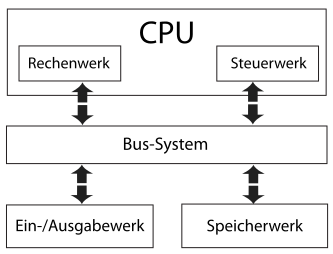
\includegraphics[scale=0.60]{Von-Neumann_Architektur}
\small Quelle: \url{https://de.wikipedia.org/wiki/Von-Neumann-Architektur#/media/File:Von-Neumann_Architektur.svg
\label{fig:vonNeumann}}
\caption{Komponenten der Von-Neumann-Architektur}
\small Quelle: Eigene Darstellung
\end{figure}

%TODO http://hki.uni-koeln.de/archive/hki2016/wisem-2011/basisinformationstechnologie-i/rechnertechnologie-i/arbeitsweise-einer-cpu-von-neumannzyklus.html
\subsection{Harvard-Architektur} 
Die Harvard-Architektur ist eine abgewandelte Form der Von-Neumann-Architektur. Der größte Unterschied besteht in der Verwaltung von Code- und Datensegement in seperaten Speichern (siehe Abbildung \ref{fig:harvard}).

\begin{figure}[!htb]
\centering
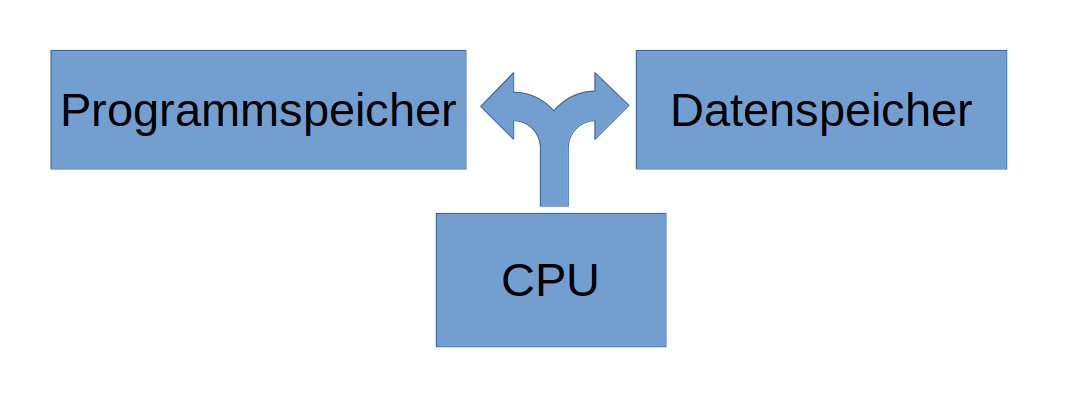
\includegraphics[scale=0.30]{harvard}
\caption{Harvard-Architektur}
\centering
\small Quelle: Eigene Darstellung
\label{fig:harvard}
\end{figure}


\noindent Diese Konzeption hat den Vorteil, dass im Gegensatz zur Von-Neumann Architektur Befehle und Daten gleichzeitig geladen werden können. Um diesen Vorteil ausnutzen zu können, benötigt ein Harvard Rechner allerdings auch getrennte Daten und Adressbusse. 
\par\bigskip
\noindent In modernen x86 Prozessoren ist eine klare Unterscheidung zwischen Von-Neumann und Harvard-Architektur nur schwer möglich. So zeigen sich eine aktuelle CPU dem Entwickler zwar als pure Von-Neumann Maschine, also mit gemeinsamen Code und Datenspeicher (RAM); allerdings besitzen sie intern einen getrennten Level-1 Cache für Instruktionen und Daten. Die beiden Architekturprinzipien haben jeweils Vor- und Nachteile, wobei in modernen Prozessoren beide Konzepte verwendet werden, um die maximale Leistung zu erzielen.
\subsection{CISC-Prozessoren}
%TODO Geschichte?
Neben den beiden vorherigen CPU-Architekturen gibt es noch zwei weitere Designphilosophien für die Entwicklung von Prozessoren, welche sich geschichtlich ergeben haben. In den Anfängen der Prozessorentwicklung gab es einige Faktoren, welche berücksichtigt werden mussten. So wurden Prozessoren bis in die 1970'er Jahre oft in Assembler programmiert. Assemblersprache ist die hardwarenäheste Methode, um Programme für Prozessoren zu entwickeln. Sie setzt das genaue Wissen über den Befehlssatz der CPU voraus. Jeder Assemblerbefehl wird in genau einen Maschinenbefehl übersetzt und dann von dem Prozessor ausgeführt. Das macht das Entwickeln in Assemblersprache sehr aufwendig. Um Entwicklern für jeden möglichen Anwendungsfall einen einzelnen Assemblerbefehl zur Verfügung stellen zu können, begannen Prozessorhersteller, immer spezialisiertere Befehle in den Befehlssatz zu integrieren.\linebreak Diese Befehle beinhalteten oft mehrere Unterschritte, zum Beispiel das Lesen aus dem Speicher und dem Verrechnen zweier Variablen. Damit ein Entwickler diese Zwischenschritte nicht eigenständig ausführen musste, wurden sie fest in den Prozessor integriert. Ein mehrstufiger Befehl wird von CISC\footnote{CISC = Complex-Instruction-Set-Computer}-Prozessoren in so genannte Mikrocodes aufgeteilt, welcher dann die einzelnen Schritte ausführt. Beispielsweise beinhaltete der Intel-486 Befehlssatz einen Befehl ''CMPXCHG  $dest,src$''\cite[S.172f]{intel4000}. Dieser vergleicht den Inhalt des Akkumulators\footnote{Der Akkumulator ist ein Register. Mehr zu Registern in Kapitel \ref{sub:register}} mit $dest$. Wenn die beiden Werte gleich sind, wird der Akkumulator mit $src$ geladen, andernfalls mit $dest$. An diesem Befehl ist zu erkennen, dass mehrere Zwischenschritte benötigt werden. Erst wird der Akku mit $dest$ verglichen und dann, je nach Ergebnis des Vergleiches, ein neuer Wert in den Akkumulator geladen. Diese Unterschritte werden mittels Microcode beschrieben, welcher fest in den Prozessor integriert ist. Dieses Konzept ermöglichte es, kompaktere Programme in Assemblersprache zu verfassen. So wuchs der Befehlssatz der Prozessoren immer weiter an und wurde komplexer. Entwickler konnten zwar kompakte Programme schreiben, mussten aber für jeden Befehl die genaue Funktion kennen, um keinen Fehler im Programmcode zu implementieren. 

%Um solche Befehle ausführen zu können, mussten die komplexen Befehle in mehrere Zwischenschritte aufgeteilt werden, welche dann vom Prozessor nacheinander abgearbeitet wurden. Prozessorhersteller entwickelten deshalb Microcode für den komplexen Befehlssatz, welche einen CISC-Befehl in mehrere Microcode Befehle dekodiert und diese ausführt. Der Befehlsdekodierer nimmt zwar auf einem Prozssor mehr Platz ein, allerdings musste somit nicht mehr oft auf den Befehlsspeicher zugegriffen werden. Durch diesen Prozess wuchs die Befehlssatzgröße stark an und wurde immer komplexer. Solch eine ISA (''Instruction Set Architecture'') wird CISC (''Complex Instruction Set Computer'') genannt.	

\subsection{RISC-Prozessoren}
Mehrere Faktoren führten dazu, dass die CISC-ISA\footnote{ISA = Instruction Set Architecture = Prozessorarchitektur} einige Nachteile aufwiesen, weshalb die RISC-ISA (Reduced Instruction Set Computer) entwickelt wurde.

\par \bigskip
\noindent Studien haben in den 1980'er Jahren gezeigt, dass 25\% der Befehle eines CISC-Prozessors 95\% der Ausführungszeit ausmachen \cite{jamil1995risc}. Das bedeutet, dass Programme den komplexen Befehlssatz, welche eine CISC CPU bot, gar nicht ausnutzten und die meiste Zeit nur simple Befehle verwendeten. \cite{patterson1985reduced} 

\par \bigskip
\noindent Ein weiterer Grund für die Entwicklung der RISC Computer war, dass die Programmierung eines Prozessors in Assemblersprache keine Notwendigkeit mehr darstellte. Mit dem Auftreten der ersten Hochsprachen, insbesondere C und ihren Compilern, mussten Entwickler nicht mehr den Befehlssatz eines Prozessors kennen. Die Compiler wandelten den Programmcode der Hochsprache erst in Assembler und daraufhin in eine maschinenlesbare Form um. Durch diese Abstraktionsschicht zwischen Prozessor und Entwickler war die kompakte Struktur von Assemblerbefehlen nicht weiter ein Entwicklungsfaktor für Prozessoren.

\par \bigskip
\noindent Daraus hat sich dann das RISC Konzept entwickelt. RISC - ''Reduced Instruction Set Computer'' - bedeutet frei übersetzt ''Prozessor mit reduziertem Befehlssatz''. Im Gegensatz zu den vorher genannten Punkten verfolgt dieser Ansatz andere Ziele. Der Befehlssatz ist auf die wesentlichen Instruktionen beschränkt. Während CISC Befehlssätze oft 200 oder mehr Befehle beinhalten, sind in RISC Befehlssätzen meist 100 oder weniger Befehle vorhanden \cite[S. 85]{TaschenbuchMikroprozessortechnik}.
\par \bigskip
\noindent Außerdem wird auf die Mikroprogrammierung verzichtet. Es werden also nicht mehr die Befehle aus dem Befehlsspeicher intern in Mikrobefehle dekodiert. Das spart auf dem Chip Fläche, da der Dekodierer keine komplexen Aufgaben mehr hat. Alle Befehle sind fest im Prozessor implementiert.
\par \bigskip
\noindent RISC-Prozessoren sollten einfach als skalare Architektur implementiert werden können. Skalar bedeutet, dass mit jedem Takt ein Befehl abgearbeitet wird. Während bei CISC-Prozessoren ein Befehl in mehrere Mikrobefehle dekodiert werden muss, wird dies bei RISC vermieden. Jeder geladene Befehl wird dekodiert und spricht genau eine Hardwareeinheit an. Komplexe Befehle, wie die bereits genannte CMPXCHG Instruktion werden nicht mehr unterstützt. Stattdessen werden die einzelnen Schritte als separate Assemblerbefehle kodiert. 

\noindent Eine weitere Eigenschaft der RISC Philosophie ist die Kommunikation mit dem Hauptspeicher nur über Load und Store Befehle. Wenn eine Variable aus dem Hauptspeicher benötigt wird, muss diese erst mit dem LOAD-Befehl in ein Register geladen werden. Durch den großen Registersatz kann diese Variable dann lange in einem Register gespeichert werden. Dadurch wird die Anzahl der Zugriffe auf den Hauptspeicher reduziert, was die Ausführungszeit senkt. In CISC Prozessoren kann eine Variable direkt mit Adresse im Hauptspeicher ohne Registereinladung verwendet werden, aber dieser komplexe Befehl muss in Microcode umgewandelt werden und benötigt bei jeder Ausführung viele Taktzyklen.\cite[S.102]{mikroprozessortechnik2011}

\par \bigskip
\noindent Da der Speicherzugriff auch in modernen Prozessoren eine zeitkritische Komponente des Funktionsmodells ist, besitzen RISC Prozessoren einen sehr großen Registersatz, üblicherweise 16 oder mehr Register. Das ermöglicht einem Programm viele seiner Variablen in den Registern zu halten, um Hauptspeicherzugriffe zu vermeiden. Hier sind allerdings die Compiler der Programmiersprachen in der Pflicht, optimierten Binärcode für RISC Prozessoren zu generieren. Alle beschriebenen Vorteile erübrigen sich, wenn sie von den Compilern nicht unterstützt werden.\linebreak Der große Registersatz muss vom Compiler auch verwendet werden, da sonst Speicherzugriffe ähnlich oft auftreten wie bei den CISC Prozessoren. \cite[S.102]{mikroprozessortechnik2011}
\par \bigskip
\noindent Moderne Prozessoren sind meist CISC Prozessoren. Mit RISC-V existiert aber ein Projekt, welches die Absicht hat, wieder moderne und konkurrenzfähige RISC Prozessorendesigns zu entwickeln und als freie ISA zur Verfügung zu stellen. 

\newpage
\section{Aufbau und Funktion}
\subsection{Register} \label{sub:register}
Register sind die schnellste Speichereinheit innerhalb einer CPU. Prozessoren besitzen eine vielfach höhere Ausführungsgeschwindigkeit als Arbeitsspeicher. Die CPU müsste ohne Register viele Taktzyklen auf Daten warten, bevor sie diese verarbeiten könnte.\cite[S.83]{elements2005}
 Register bieten deshalb die Möglichkeit, sehr kleine Datenmengen mit einer sehr geringen Latenz prozessorintern lesen und schreiben zu können. Übliche Registergrößen sind 8,16,32 oder 64 Bit. Sie werden aus Flip-Flops aufgebaut, welche jeweils genau ein Bit speichern können. Das heißt ein 64 Bit Register besteht aus 64 gemeinsam gesteuerten Flip-Flops. Diese Art der Datenspeicherung hat allerdings auch einige Nachteile. So verbrauchen Register sehr viel Energie und Platz auf dem Prozessorchip. Es wird deshalb sehr wenig Registerspeicher in Prozessoren verbaut.\cite[S.89]{mikroprozessortechnik2011}

\subsubsection{Aufbau}
Register bestehen aus so genannten Flip-Flops. Diese Schaltungen können genau ein Bit speichern. 

\begin{figure}[!htb]
\centering
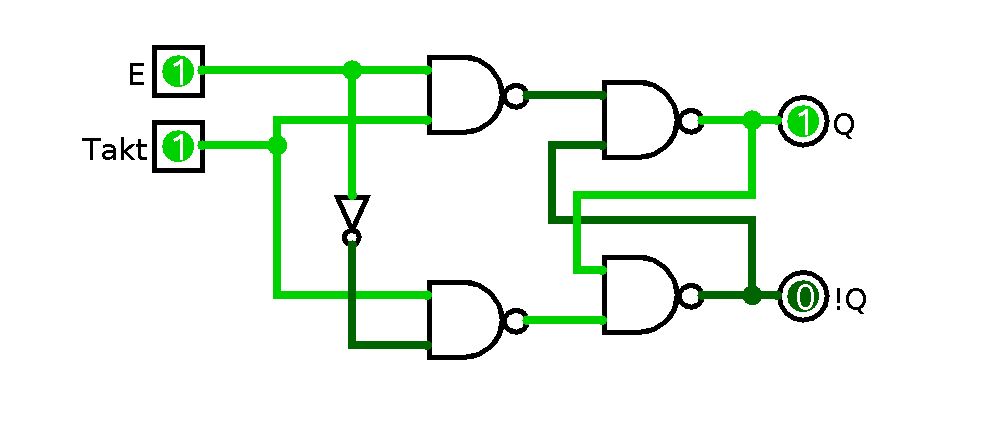
\includegraphics[scale=0.30]{flipflop}
\caption{Schaltnetz D-Flip-Flop}
\centering
\small Quelle: Eigene Darstellung
\label{fig:flipflop}
\end{figure}

\noindent In Abbildung \ref{fig:flipflop} ist das Schaltnetz eines D-Flip-Flops dargestellt. Es ist aus 4 NAND Gattern aufgebaut und speichert den Wert des Eingangs (E), wenn der Takt auf 1 steht. Ein NAND Gatter ist ein UND Gatter dessen Ausgang negiert wird. Der Ausgang eines AND-Gatters ist 1, wenn alle Eingänge ebenfalls 1 sind. Umgekehrt gilt, wenn alle Eingänge eines NAND-Gatters auf 1 stehen, so wird der Ausgang den Wert 0 besitzen.\cite[S.12-14]{elements2005}

\noindent In Tabelle \ref{andnand} sind die Schaltregeln für ein AND und NAND Gatter dargestellt.\linebreak Ein FlipFlop kann allerdings nur ein Bit speichern, deshalb werden für ein Register mehrere Flip-Flops zusammengeschaltet und agieren damit als gemeinsamer Speicher. In Abbildung \ref{fig:4bitreg} auf Seite \pageref{page:4bitreg} sind vier solcher D-Flip-Flops zu einem 4-Bit Register verbunden worden.  Aktuelle Prozessoren besitzen meist mindestens 64-Bit Register oder sogar mehr\footnote{Mit dem Intel AVX Befehlssatz wurde die Breite der SIMD-Register von 128 auf 256 Bit erhöht\cite{lomont2011introduction}}. Durch die hohe Anzahl an benötigten Gattern ergibt sich ein sehr hoher Stromverbrauch und eine beachtliche Wärmeentwicklung. Aus diesem Grund sind Register die kleinste, aber dafür schnellste Speichereinheit in einem Prozessor.

\begin{table}[!htb]
\centering
\begin{tabular}{|c|c|c|c|}
\hline
Eingang 1 & Eingang 2 & AND & NAND \\ \hline
0         & 0         & 0   & 1    \\ \hline
0         & 1         & 0   & 1    \\ \hline
1         & 0         & 0   & 1    \\ \hline
1         & 1         & 1   & 0    \\ \hline
\end{tabular}
\caption{Schaltregeln AND und NAND Gatter}
\label{andnand}
\centering
\small Quelle: Eigene Darstellung
\end{table}


\newpage
\label{page:4bitreg}
\begin{figure}[!htb]
\centering
\caption{Schaltnetz 4-Bit Register}
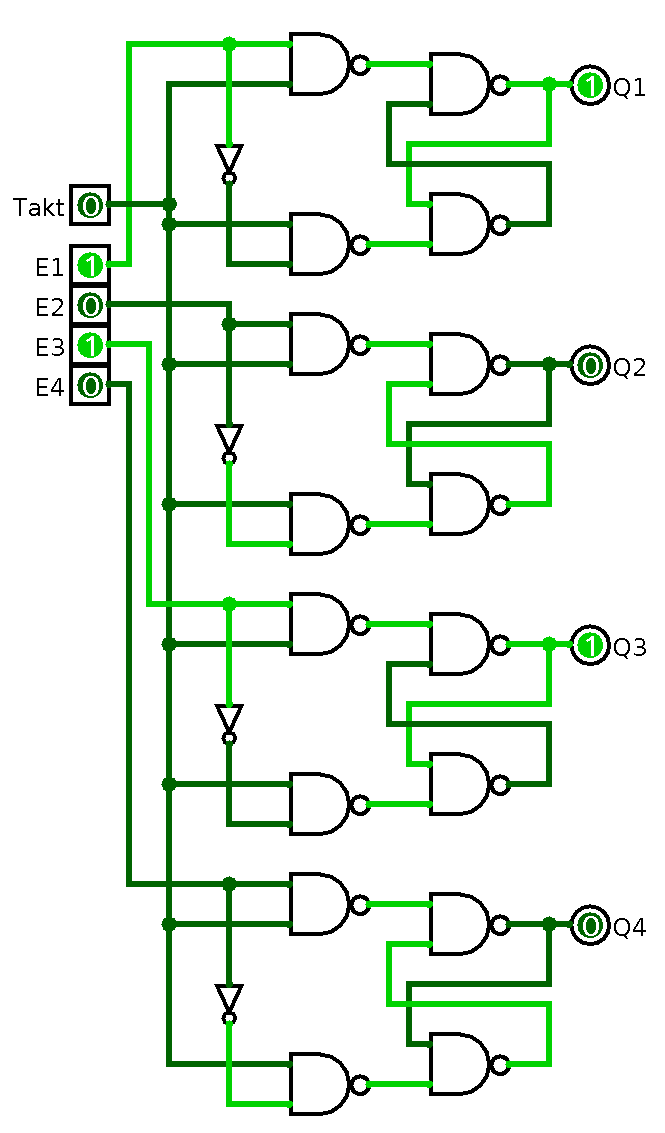
\includegraphics[scale=0.35]{4bitreg}
\small Quelle: Eigene Darstellung
\label{fig:4bitreg}
\end{figure}
\newpage


\subsubsection{Universalregister}
Es werden zwei Arten von Registergruppen unterschieden. Universalregister und Spezialregister. In einem Universalregister können beliebige Daten gespeichert werden. Sie sind einem Entwickler zugänglich, das heißt, er kann auf jedes Universalregister direkt zugreifen und seinen Wert verändern. 

%\begin{figure}[!htb]
%\centering
%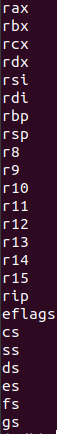
\includegraphics[scale=0.5]{inforeg}
%\caption{Ausgabe des GDB-Befehls ''info registers''}
%\centering
%\label{fig:inforeg}
%\end{figure}


\begin{wrapfigure}{L}{0.3\textwidth}
\centering
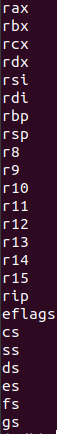
\includegraphics[scale=0.5]{inforeg}
\centering
\caption{Ausgabe des GDB-Befehls ''info registers''}
\label{fig:inforeg}
\small Quelle: Eigene Darstellung
\end{wrapfigure}

\noindent Abbildung \ref{fig:inforeg} zeigt die Register des Prozessors i7-6700HQ. Ausgenommen sind hier die Register für spezielle Befehlssatzerweiterungen wie zum Beispiel SIMD oder AVX. Diese sind in der Regel 128 bzw. 256 Bit breit. Die Universalregister sind in Abbildung \ref{fig:inforeg} mit den Namen R8 bis R15 zu sehen.
\subsubsection{Spezialregister}
Spezialregister werden von einer CPU für interne Zwecke genutzt. Oft sind in Prozessoren ähnliche Spezialregister zu finden. 

\par \bigskip
\noindent Der Stack Pointer(SP) ist ein Register, welches auf die aktuelle Position des Stacks im Speicher zeigt. Der Stack ist ein Stapelspeicher, er verlangt also keine Adressierung mittels Adressen. Er wird mit den beiden Befehlen PUSH und POP angesteuert. PUSH schiebt einen Wert aus einem Register auf den Stack, POP lädt den obersten Wert in ein Register.  Wenn der Befehl zur Speicherung eines Werts auf dem Stack ausgeführt wird, inkrementiert die CPU automatisch den Wert des Stack Pointers. Dadurch zeigt das Register immer auf die nächste freie Speicheradresse im Stack.

\par \bigskip
\noindent Der Instruction Pointer (IP) enthält die Adresse des nächsten Befehls im Programmspeicher der ausgeführt werden muss. Auch er wird nach der Abarbeitung eines Befehlszyklus als letzter Schritt inkrementiert. Dieses Register bietet allerdings die Möglichkeit, einen anderen Wert zu laden. Das wird zur Realisierung von Sprüngen innerhalb des Programmcodes benötigt. 

\par \bigskip
\noindent Das Statusregister (SR) wird zur Ausführung von bedingten Sprunganweisungen gebraucht.\newline Es wird auch Flagregister genannt, da die ALU, in Abhängigkeit der zuletzt ausgeführten Rechenoperation, einzelne Bits (Flags) setzen kann. Auf die einzelnen Flags und ihre Bedeutung wird im Abschnitt der ALU (siehe \ref{subsec:alu}) näher eingegangen

\subsection{Steuerwerk}
Das Steuerwerk ist für die Steuerung der internen Bussysteme des Prozessors zuständig. Im Befehlsregister (Instruction Pointer bzw. IP) ist die Adresse des nächsten Befehls enthalten, welcher ausgeführt werden soll. Der Befehl wird von der Adresse des Befehlsregisters in den Befehlsdekodierer geladen und analysiert. Falls nötig, wird der Befehl in mehrere Schritte unterteilt, die nacheinander abgearbeitet werden müssen. Ob und wie viele solcher Schritte benötigt werden, um einen bestimmten Befehl auszuführen, bestimmt zum einen die Architektur des Prozessors und zum anderen der Befehl an sich. Bei RISC Prozessoren ist keine weitere Unterteilung in mehrere Befehle notwendig, bei CISC Prozessoren besitzt der Befehlssatz sehr viel kompliziertere Befehle, welche nicht in einem Takt abgearbeitet werden können. Hier wird der Befehlsdekodierer den Befehl in die nötigen Teilbefehle umwandeln und nacheinander ausführen.

\par\smallskip\noindent Da über ein Bussystem immer nur zwei Komponenten miteinander kommunizieren können, muss das Steuerwerk die Busse für die jeweiligen Komponenten freischalten. 


\subsection{Arithmetisch Logische Einheit} \label{subsec:alu}
%https://en.wikibooks.org/wiki/Microprocessor_Design/ALU#Example:_4-Bit_ALU
%https://en.wikibooks.org/wiki/Microprocessor_Design
Die ALU (Arithmetic Logic Unit) ist der Teil einer CPU, welcher die eigentliche Datenverarbeitung durchführt. Sie verfügt über keinen eigenen Speicher, die Ergebnisse müssen in Registern gespeichert werden. Die ALU ist ein Schaltwerk, welches einfache Operationen auf meist zwei Operanden ausführen kann. So kann das Rechenwerk einer CPU meistens arithmetische, logische und bitschiebende Operationen ausführen. Arithmetische Operationen umfassen Addition und Subtraktion, seltener auch Multiplikation und Division. Addierer und Subtrahierer sind als Hardwareeinheit in die ALU integriert, wohingegen Multiplikation und Division meist algorithmisch durchgeführt werden. Die ALU alleine hat wenig Wirkung, sie obliegt der Kontrolle des Steuerwerkes. Dieses steuert, welche Operation ausgeführt wird, mit welchen Operanden sie ausgeführt wird und in welches Register das Ergebnis gespeichert werden soll.

\par \bigskip
\noindent Rechenwerke sind innerhalb eines Prozessors oft unterschiedlich aufgebaut. 
Sehr einfache Prozessoren besitzen häufig ein spezielles Register, in dem das Ergebnis einer ALU Operation automatisch gespeichert wird. Dieses Register wird Akkumulator genannt. Solch ein Register hat den Vorteil, dass auf die Angabe eines Zieles bei der Programmierung verzichtet werden kann, da der Ausgang der ALU fest mit dem Akkumulator verbunden ist. Des weiteren ist der Ausgang des Akkumulators fest mit einem der zwei Eingänge der ALU verbunden. Man kann sich den Akkumulator also als fest vorgeschaltetes Register des Rechenwerks vorstellen, in dem auch das Ergebnis gespeichert wird. Deshalb muss bei einer Rechenoperation vom Programmierer nur ein Operand angegeben werden. 

\par\bigskip\noindent \textbf{Beispiel:} Im Akkumulator befindet sich der Wert 10d  und der Assemblerbefehl ADD RAX wird ausgeführt. Dann wird die ALU vom Steuerwerk angewiesen, eine Addition auszuführen und übergibt als Parameter am zweiten Eingang den Wert des Registers RAX. Der erste Eingang ist mit dem Akkumulator verbunden und übergibt deshalb den Wert 10d. Das Ergebnis der Berechnung wird wiederum in den Akkumulator gespeichert und überschreibt den vorherigen Wert 10d.  

\noindent Diese feste Konfiguration der ALU hat allerdings einige Nachteile, weshalb in den meisten modernen Prozessoren eine ALU implementiert ist, die mit keinem Register fest verbunden ist. Eine Rechenwerksoperation muss dann immer zwei Quellregister und ein Zielregister angeben. Diese Konfiguration ist zwar sehr flexibel in der Übergabe der Speicherorte, allerdings benötigt sie zusätzliche Schaltungslogik auf dem Chip und die Codekomplexität nimmt zu.

\par\bigskip
\noindent \textbf{Beispiel:} Bei der Ausführung des Befehls ADD RAX, RBX, RCX werden die Werte der beiden Register RAX und RBX addiert und das Ergebnis in RCX gespeichert.

\par\smallskip\noindent Die ALU speichert zwar das Ergebnis in dem ihr zugewiesenen Register, allerdings kann der Prozessor keine Eigenschaften der letzten Operation unterscheiden. Diese Fähigkeit wird aber benötigt, wenn der Entwickler anfordert, dass das Programm an eine andere Adresse springt, sollte das letzte Rechenergebnis 0 ergeben haben. In Hochsprachen entspricht dieser Anwendungsfall zum Beispiel einer if-Bedingung. Wenn die Bedingung erfüllt ist, wird ein gesonderter Codeteil ausgeführt. Damit der Prozessor diese Bedingung prüfen kann, ist den meisten Prozessoren ein Statusregister integriert. Das Statusregister speichert nicht wie die Universalregister einen Wert ab, der als Binärzahl interpretiert wird, sondern jedes Bit im Register steht für eine bestimmte Eigenschaft der vorhergehenden Rechenoperation. Diese Bits werden Flags genannt.\newline Eine 1 bedeutet, dass die letzte Operation diese Bedingung erfüllt hat, eine 0 das Gegenteil. Welche Flags ein Prozessor unterstützt und wie diese angeordnet sind unterscheidet sich von Prozessor zu Prozessor. Allerdings sind die fünf grundlegensten Flags in fast allen Prozessoren implementiert.

\par\smallskip\noindent \textbf{Zero-Flag (Nullbit):} Das Zero-Flag ist sehr simpel aufgebaut. Wenn das letzte Ergebnis der ALU Null war, wird das Bit auf 1 gesetzt, ansonsten auf 0. Mit diesem Flag lässt sich zum Beispiel die Abbruchbedingung für eine Schleife leicht prüfen. Die Anweisung: $$for(int \ i=5;i \ > \ 0;i--)\{\}$$ wird solange durchlaufen, bis das Ergebnis der ALU Operation ($i$ -\ -) gleich Null ist und damit das Zero-Flag gesetzt wird. Dann wird die Schleife abgebrochen und der Programmablauf fortgesetzt. \cite[S.95]{mikroprozessortechnik2011}
\begin{table}[!htb]
\centering
\begin{tabular}{|c|c|c|}
\hline

i & Zero-Flag & Nächster Schritt \\ \hline
5 & 0         & Weiter           \\ \hline
4 & 0         & Weiter           \\ \hline
3 & 0         & Weiter           \\ \hline
2 & 0         & Weiter           \\ \hline
1 & 0         & Weiter           \\ \hline
0 & 1         & Abbruch          \\ \hline
\end{tabular}
\caption{Schritte der for-Schleife}
\label{forschleife}
\small Quelle: Eigene Darstellung
\end{table}

\noindent Tabelle \ref{forschleife} zeigt die Nutzung des Zero-Flags zur Prüfung der Abbruchbedingung der for-Schleife. 

\par\bigskip\noindent \textbf{Carry-Flag (Übertragsbit):} Das Carry-Flag zeigt an, ob es bei der letzten ALU-Operation zu einem Übertrag gekommen ist. Wie in Tabelle \ref{tab:uebertrag} bereits dargestellt, kommt es zu einem Übertrag, wenn das Ergebnis nicht mehr korrekt mit der zur Verfügung stehenden Bitbreite dargestellt werden kann.\cite[S.95]{mikroprozessortechnik2011}


\begin{table}[!htb]
\centering
\begin{tabular}{|c|c|c|c|}
\hline
Rechnung & Ergebnis (d) & Ergebnis (b) & Carry-Flag \\ \hline \hline
253+2    & 255          & 11111111     & 0          \\ \hline \hline
253+3    & 256          & 00000000     & 1          \\ \hline
\end{tabular}
\caption{Beispiele Carry-Flag}
\label{tab:carry}
\small Quelle: Eigene Darstellung
\end{table}




\noindent In Tabelle \ref{tab:carry} sind beispielhaft zwei Rechenoperationen dargestellt. Es wird angenommen, dass die Operation von einer 8-Bit ALU ausgeführt wird. In der ersten Zeile wird die Summe aus 253 und 2 berechnet. Das Ergebnis kann gerade noch als 8-Bit Dualzahl dargestellt werden ($11111111b = 255d$), das Carry-Bit wird deshalb nicht von der ALU gesetzt. Das Ergebnis der Rechnung in der zweiten Zeile  würde neun Bits benötigen um korrekt dargestellt werden zu können ($100000000b = 256d$). Da das Rechenwerk aber nur eine Breite von 8 Bit hat wird im Zielregister der Wert der ersten 8 Bit des Ergebnisses, also null gespeichert. Um diese fehlerhafte Rechnung anzuzeigen, wird nun das Carry Bit im Flagregister gesetzt.  
Sollte der letzte ausgeführte ALU Befehl ein Schiebebefehl gewesen sein, so wird das Carry Flag dazu verwendet, den Wert des herausgeschobenen Bits anzuzeigen.

\par\bigskip\noindent \textbf{Sign-Flag (Vorzeichenbit):} Das Vorzeichenbit entspricht dem MSB (most significant bit) des Ergebnisses. Das MSB ist das höchstwertige Bit einer Dualzahl.

 \par\bigskip\noindent \textbf{Overflow-Flag (Überlauf-Bit):} Diese Flag wird beim Rechnen mit Zahlen im Zweierkomplement benötigt. Es wird gesetzt, wenn bei einer Addition oder Subtraktion ein Übertrag auf das MSB stattfindet, also das höchstwertige Bit verändert wird. 
\begin{table}[!htb]
\centering
\begin{tabular}{|c|c|c|c|}
\hline
Rechnung (d) & Ergebnis (Zweierkomplement) & Ergebnis (b) & Overflow-Flag \\ \hline 
122+5        & 127                         & 01111111     & 0            \\ \hline 
122+6        & -128                        & 10000000      & 1            \\ \hline

\end{tabular}
\caption{Rechnen im Zweierkomplement mit 8-Bit Zahlen}
\small Quelle: Eigene Darstellung
\label{tab:overflow}
\end{table}

\noindent In Tabelle \ref{tab:overflow} sind zwei Rechnungen dargestellt. Im Zweierkomplement hat eine Zahl mit $n$ Bits folgenden darstellbaren Zahlenbereich: 
$${-2}^{n-1}+ ... +2^{n-1}-1$$
In Tabelle \ref{tab:overflow} wird mit 8-Bit Zahlen gearbeitet, also reicht der darstellbare Zahlenbereich für das Beispiel von $-128$ bis $+127$. Die erste Rechnung ergibt 127, die höchste positive darstellbare Zahl im Zweierkomplement mit 8-Bit. Es kommt zu keinem Übertrag auf das MSB, also wird das Overflow Bit nicht gesetzt. In der zweiten Zeile kommt es zu einem Übertrag auf das MSB und das Ergebnis wird verfälscht, da +128 nicht mehr im darstellbaren Zahlenbereich für diese Rechnung liegt. Um das falsche Ergebnis anzuzeigen wird die ALU das Overflow Bit auf 1 setzen. 
%TODO Overflow Flag wird mit XOR aus Carry in und Carry Out berechnet ... Noch nicht ganz verstanden.


\subsection{Bussysteme}
Bisher wurde der Aufbau und die Funktion der einzelnen Komponenten einer CPU erläutert, aber nicht wie die Kommunikation innerhalb eines Prozessors abläuft. Wie teilt zum Beispiel das Steuerwerk dem Rechenwerk mit, dass eine Rechnung auszuführen ist? Prinzipiell könnte jede Komponente mit jeder anderen verbunden werden. Das Steuerwerk hätte dann jeweils zwei Leitungen zum Rechenwerk, Registerwerk und zum Cache, eine für jede Datentransportrichtung. Wenn alle Komponenten auf diese Weise verbunden wären, ergäbe das ein enorm kompliziertes Chipdesign mit schlechter Energieeffizienz. Dazu kommt die nicht vorhandene Konnektivität zu externen Schnittstellen. Man müsste jeden externen Baustein an alle Komponenten des Prozessors anschließen\cite[S.62]{mikroprozessortechnik2011}. Um all diese Probleme lösen zu können, wurde der Systembus in den Prozessor eingefügt. Die Idee dahinter ist, dass alle Komponenten an einen zentralen Kommunikationskanal angeschlossen sind. Man unterteilt diesen in Datenbus, Steuerbus und Adressbus \cite[S.62]{mikroprozessortechnik2011}. Der Vorteil dieser Architektur besteht darin, dass externe Schnittstellen sehr einfach in die Prozessorkommunikation integriert werden können. Aber auch dieses Konzept stellt gewisse Anforderungen an den Zugang zu diesem gemeinsam genutzten Systembus. Es muss sichergestellt werden, dass zu jeder Zeit nur ein Baustein senden darf, sonst kommt es zu Kollisionen auf dem entsprechenden Bus. In einem Prozessor wird diese Aufgabe von einem so genannten Busmaster übernommen. Er steuert, welcher Baustein wann auf welchen Bus zugreifen  und Daten senden bzw. empfangen kann.
\par\smallskip\noindent
Eine wichtige Entscheidung bei der Entwicklung eines Prozessors ist die Breite der Busse. Der Adressbus zum Beispiel limitiert mit der Breite $n$ den möglichen adressierbaren Speicherplatz auf $2^n$ Speicherplätze. Ein 32-Bit breiter Adressbus kann $2^{32} = 4.294.967.296$ Speicherplätze mit jeweils 8-Bit Breite ansprechen, also etwa 4 Gigabyte. Diese Limitierung war der ausschlagebende Grund, den Adressbus zu erweitern, da 4 Gigabyte Hauptspeicher nicht mehr ausreichten. 


\newpage
\section{Speicherverwaltung}
Am Anfang der Prozessorentwicklung war Hauptspeicher nur in kleinen Kapazitäten verfügbar. Ein Programm war häufig zu groß, um komplett in den Hauptspeicher geladen zu werden. Deshalb wurden sogenannte Overlays verwendet. Wenn ein Programm geladen werden sollte, wurde ein Bereich im Hauptspeicher für Overlays reserviert. Der Entwickler musste dann sein Programm in Segmente (Overlays) unterteilen und diese während der Laufzeit nacheinander in den Hauptspeicher zur Ausführung laden. Diese Speicherverwaltungsmethode hatte aber Nachteile. Der Entwickler musste neben seinem geschriebenen Programm auch noch auf die Speicherverwaltung achten, was höheren Arbeitsaufwand verursachte. Außerdem erhöhte das ständige Nachladen von Overlays in den Speicher die Ausführungszeit erheblich. \cite[S.173]{mikroprozessortechnik2011}


\par\bigskip\noindent Um die Programmierer von der zeitraubenden Arbeit der manuellen Speicherverwaltung zu entlasten, hat sich das System des virtuellen Speichers etabliert. Dabei sieht der Programmierer nur einen großen zusammenhängenden Speicherbereich und muss keine Rücksicht auf die Größe des Hauptspeichers nehmen. Sollte ein Programm mehr Hauptspeicher benötigen als physisch in dem System vorhanden ist, dann wird das Betriebsystem die Daten auf ein anderes Speichermedium auslagern. Diese Technik wird Paging genannt und muss vom Betriebssystem unterstützt werden.

\subsection{Paging}
Um dieses Prinzip zu veranschaulichen, ist folgendes Beispiel hilfreich. 
\par\smallskip\noindent Ein Entwickler hat ein Programm geschrieben, welches 4 MiByte (4096 KiByte) Arbeitsspeicher benötigt. Das System, auf welchem das Programm ausgeführt werden soll, besitzt allerdings nur 1 MiByte (1024 KiByte) physischen Hauptspeicher. Wenn das Betriebssystem Paging unterstützt, wird es folgendermaßen vorgehen:
\par\smallskip\noindent Das Betriebssytem teilt den benötigten Adressraum von 4 MiByte in vier gleich große Teile (jeweils 1024 KiByte) ein, welche einzeln in den Hauptspeicher geladen werden können. Diese Speicherfenster nennt man ''Page Frames''. Zum Start des Programmes wird eines der vier Pageframes in den Hauptspeicher geladen und der Rest auf einem Massenspeicher gespeichert. Die Seiten werden vom Betriebssystem in einer Seitentabelle (''Page-Table'') verwaltet.  In Abbildung \ref{fig:paging} ist dieses Beispiel dargestellt. 4 MiByte virtueller Hauptspeicher stehen zur Verfügung.\newline Allerdings ist nur das erste Page-Frame physisch im Hauptspeicher. Die restlichen drei Page-Frames sind im Massenspeicher hinterlegt und werden bei Bedarf geladen.\cite[S.113ff]{rechnerarchitektur}

\begin{figure}[!htb]
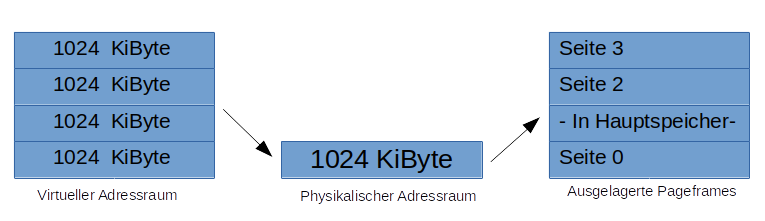
\includegraphics[scale=0.7]{Paging}
\caption{Paging}
\centering
\label{fig:paging}
\end{figure}

\noindent Fordert das Programm nun eine virtuelle Adresse an, welche nicht im physikalischen Speicher liegt, wird die Ausnahme Seitenfehler (''Pagefault Exception'') ausgelöst. Bei einer Exception wird eine Behandlungsroutine angestoßen, ähnlich den Interrupts. Im Unterschied zu Interrupts wird eine Exception von der CPU selbst ausgelöst. Im Falle dieser Ausnahme wird die Routine die Seite (''Page Frame''), welche die benötigte Adresse enthält, aus dem Massenspeicher in den Hauptspeicher laden. Paging ist ein kompliziertes Verfahren, um das Zusammenspiel von virtuellen und physischen Speicher zu verwalten. Dieses Konzept in Software zu realisieren würde wie die Overlays zu viel Leistung kosten. Deshalb besitzen die meisten modernen Prozessoren einen Controller für solche Speicherverwaltungsaufgaben, die so genannte MMU (''Memory Management Unit''). \cite[S.177ff]{mikroprozessortechnik2011}



\subsection{Cache} \label{subsec:cache}
Zum Beginn der Prozessorentwicklung entsprach der Speichertakt in etwa dem eines Prozessors. Allerdings zeigte sich schnell, dass der Speichertakt nicht mit dem Prozessortakt in gleichem Maße steigen kann. Der daraus entstandene Geschwindigkeitsunterschied wird auch Speichermauer (''Memory Wall'') genannt \cite{mckee2004reflections}.
%Quelle PDF http://www.cs.columbia.edu/~sedwards/classes/2012/3827-spring/advanced-arch-2011.pdf
Das war ein Problem für die Prozessorentwickler. Mit zunehmenden Leistungsunterschied zum Speicher muss der Prozessor mehrere Taktzyklen warten,  bis der Speicher auf eine Anforderung antwortet.\cite[S.180]{mikroprozessortechnik2011} Die Kommunikation mit Speichermedien ist allerdings ein elementarer Bestandteil der Funktionsweise eines Prozessors. Um diese Latenzzeiten zumindest verkürzen zu können, wurde ein weiterer Speichermechanismus zwischen Registerwerk und Arbeitsspeicher eingeführt, der Cache.\newpage\noindent Der Cache ist im Prozessor selbst verbaut und hat üblicherweise nur eine Größe von drei bis sechs Megabyte, da er sehr viel Platz und Strom verbraucht. Dafür ist er um ein vielfaches schneller als der Arbeitsspeicher. Der Cache selbst ist wiederum in meist drei Teile unterteilt. Der sogenannte Level-1-Cache ist der schnellste Speicher im Cachesystem. Er ist meistens an den Prozessortakt angeschlossen und hat deshalb eine den Registern ähnliche Latenzzeit. Gleichzeitig ist er aber auch der kleinste Speicher in der Cacheorganisation. 
Üblicherweise ist er zwischen 8 und 32 KByte groß. Eine Besonderheit des Level-1-Caches ist, dass er  einen getrennten Daten und Instruktionsspeicher besitzt. Etwas mehr Speicherplatz bietet der Level-2-Cache. Er besitzt ca. 256 KByte Speicherplatz, wird aber mit geringerem Takt betrieben. Daraus folgen erhöhte Latenzzeiten im Gegensatz zum L1-Cache. Den größten Speicherplatz bietet der Level-3-Cache. Dieser besitzt eine Größe von etwa 6 MByte\footnote{Diese Größen basieren beispielhaft auf einem Intel i7-6700HQ. Serverprozessoren besitzen ein vielfaches mehr Cache}. Der L3 Cache taktet sehr viel langsamer als der Prozessor und hat deshalb auch die höchsten Latenzzeiten innerhalb der Cacheorganisation.\cite{molka2009memory}. Hier ist noch anzumerken, dass bei Mehrkernprozessoren der Level-3-Cache zwischen allen Kernen geteilt wird, wohingegen der Level-1 sowie Level-2-Cache jedem Kern exklusiv zu Verfügung steht.


\begin{figure}[!htb]
\centering
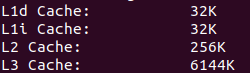
\includegraphics[scale=0.5]{lscpu}
\caption{Teil der Ausgabe des Befehls ''lscpu'' unter Ubuntu}
\centering
\label{fig:lscpu}
\small Quelle: Eigene Darstellung
\end{figure}

\noindent In Abbildung \ref{fig:lscpu} ist als Beispiel die Cache-Organisation eines Intel i7-6700HQ Notebookprozessors dargestellt. Gut zu sehen ist, dass der L1 Cache in einen Datenspeicher (''L1d'') und einen Instruktionsspeicher (''L1i'') geteilt ist. 

\noindent Er ist also nicht imstande, einen Ersatz für den Arbeitsspeicher bereitzustellen. Durch statistische Untersuchungen von Speicherzugriffen konnten allerdings bestimmte Erkenntnisse gewonnen werden. Wenn ein Prozessor Daten aus dem Arbeitsspeicher anfordert, ist die Wahrscheinlichkeit groß, dass er in kommenden Speicherzugriffen Daten anfordern wird, welche in der Nähe der vorher verwendeten Adresse liegen. Diesen Umstand nennt man räumliche Lokalität. Dies tritt beispielsweise ein, wenn Textdaten unfragmentiert im Arbeitsspeicher vorhanden sind. Dann wird der Prozessor mit hoher Wahrscheinlichkeit sequentiell einen ganzen Block im Arbeitsspeicher anfragen. Der Cache wird daraufhin den Datenblock aufnehmen, um die Latenz der kommenden Anfragen zu verbessern. 

\noindent Eine weitere Eigenschaft ist die zeitliche Lokalität des Speicherzugriffs. Wenn eine Adresse aus dem Hauptspeicher angefordert wird, so ist die Wahrscheinlichtkeit höher, dass sie bald wieder benötigt wird. Solch eine Situation kann zum Beispiel bei dem Überprüfen einer Laufvariablen in einer Schleife auftreten. Anstatt die Adresse bei jedem Schleifendurchlauf aus dem langsamen Hauptspeicher zu laden, wird sie im Cache gespeichert. 
Der Cache Speicher ist wie der Arbeitsspeicher ein flüchtiger Speicher, er verliert also seinen gespeicherten Inhalt bei Stromverlust. Daraus folgt auch, dass er zu Beginn leer ist und sukzessive mit Einträgen gefüllt werden muss.\cite[S.180-188]{mikroprozessortechnik2011}
\subsubsection{Cacheorganisation}
Vereinfacht dargestellt besteht der Cache aus so genannten Cachezeilen (''Cache-Lines''). Diese Cachezeilen haben eine bestimmte Blocklänge (''block size'')\cite[S.183]{mikroprozessortechnik2011}. Wenn Daten in den Cache geladen werden, dann immer in diesen festen Blöcken. Auch wenn der Prozessor nur eine Adresse aus dem Arbeitsspeicher benötigt, wird im Cache, falls nicht schon vorhanden, der ganze Block in dem sich diese Adresse befindet in eine Cachezeile gespeichert.
\subsubsection{Ersetzungsstrategien}
 Wie bereits in Kapitel \ref{subsec:cache} beschrieben ist die Speicherkapazität von Cache-Speicher aufgrund des hohen Stromverbrauchs und Platzbedarfs sehr begrenzt. Deshalb kann es passieren, dass der Cache voll ist und keine weiteren Einträge aufnehmen kann. Um solche Ausnahmen zu behandeln, wurden verschiedene Cache-Ersetzungsstrategien implementiert. Der Fokus bei diesen Strategien liegt darauf, diejenigen Cache Zeilen zu ersetzen, welche die geringste Wahrscheinlichkeit aufweisen, wieder verwendet zu werden. Es wird also immer versucht, die Wahrscheinlichkeit für Cache-Treffer zu maximieren, um die Wartezeit des Prozessors auf Daten oder Instruktionen zu minimieren. \cite[S.187]{mikroprozessortechnik2011}


%---------------FIFO-----------------------------
\noindent Die einfachste Cache Ersetzungsstrategie ist die FIFO-Ersetzung (''First In-First out''). Bei ihr wird der älteste Cache Eintrag mit dem neuesten überschrieben. Da der älteste Cache Eintrag lange nicht mehr benutzt wurde, ist stochastisch davon auszugehen, dass seine Ersetzung mit einem aktuellen Eintrag in einer erhöhten Cache-Treffer Wahrscheinlichkeit resultiert.

%---------------LFU------------------------------------
\noindent Eine weitere Ersetzungsstrategie ist die LFU-Ersetzung (''Least Frequently Used''). Im Gegensatz zur FIFO-Ersetzung wird hier über eine bestimmte Zeitspanne der Cache überwacht und dann die Cachezeile überschrieben, welche die geringste Nutzungszahl aufweist. Auch hier ist es wieder günstiger, diese Cachezeile mit neuen Daten zu überschreiben, da die alte seltener benutzt wurde und somit der Zeitverlust beim erneuten Laden aus dem Hauptspeicher vertretbar ist.

%--------------Random----------------------------------------
\noindent Das Zufallsprinzip erfordert im Gegensatz zur LRU-Ersetzung keine gesonderte Logik zur Bestimmung der zu löschenden Zeile. Der neue Cache-Eintrag wird einfach über eine zufällig ausgewählte Cache-Zeile geschrieben. Diese Methode mag zwar ungewöhnlich erscheinen, aber es wurde gezeigt, dass das zufällige Ersetzen von Cachezeilen mit neuen Einträgen unter Umständen bessere Ergebnisse als die anderen Strategien liefern kann.\cite[S.185ff]{mikroprozessortechnik2011} \cite{smith1985instruction}

\addtocontents{toc}{\protect\newpage}

\newpage
\section{Programmablauf}	\label{sec:programmablauf}
\subsection{Schleifen}
Programmschleifen sind für jedes Programm von essentieller Bedeutung und in jeder modernen Programmiersprache implementiert. Ohne sie wäre kein effizienter und kompakter Programmaufbau möglich. In Hochsprachen sind zwei Grundlegende Arten von Schleifen geläufig. Zum einen die Schleifen mit festgelegter Anzahl an Durchläufen: 
$$for(int \ i=0; i<100; i++)\{...\}$$
Diese Schleife wird genau 100 mal durchlaufen, bis sie abbricht. Zum anderen gibt es auch Szenarien, in welchen die benötigte Zahl an Durchläufen nicht bekannt ist:
$$while(''Bedingung'')\{...\}$$
Diese Schleifen werden solange durchlaufen, bis die Abbruchbedingung ''true'' ergibt. Die gezeigten Beispiele entsprechen Schleifen in einer Hochsprache, aber wie werden diese Konstrukte auf der Hardware durch die CPU ausgeführt?
Prozessoren durchlaufen grundlegend einen linearen Programmablauf. Sie holen sich den nächsten Befehl aus der Speicherzelle, auf dessen Adresse der Instruction Pointer (IP) zeigt. Diesen Befehl dekodieren sie und führen ihn aus. Daraufhin wird der Wert des IP inkrementiert, damit er auf den nächsten Befehl im Speicher zeigt. Um Schleifen realisieren zu können, besitzen Prozessoren spezielle Befehle, mit denen sie den Wert des IP ändern können. Diese Befehle werden Sprungbefehle (''Jump'') genannt. Der Jump-Befehl lädt den Instruction Pointer mit einer angegebenen Adresse. Das bedeutet, dass der Programmablauf an der neuen Adresse weitergeführt wird. Im Grunde muss bei einer Schleife ein bestimmter Codeabschnitt immer wieder durchlaufen werden. Zur Veranschaulichung wird nun eine einfache Schleife in der Hochsprache C mit dem daraus erzeugten Assemblercode für einen Intel Prozessor verglichen. Kompiliert wurde der Code unter Ubuntu 17.10 mit dem Linux-Kernel 4.13.

\begin{code}[!htb]
\begin{lstlisting}
int main(int argc, char const *argv[])
{
	unsigned int counter = 0;
	while(counter<100){
		counter++;
	}
	return 0;
}
\end{lstlisting}
\caption[C Code einfache Schleife]{C-Code für eine einfache Schleife}
\centering
\small Quelle: Eigene Darstellung
\label{code:scheife}
\end{code}
\newpage
\par\bigskip\noindent Das Programm, welches im Codeblock \ref{code:scheife} dargestellt ist, initialisiert eine Variable ''counter'' mit dem Wert 0 und inkrementiert diesen in einer Schleife so lange, bis er den Wert 100 erreicht. Der Assemblercode für dieses Programm ist folgendermaßen aufgebaut (Codeblock \ref{code:scheifeasm}):


\begin{code}[!htb]
\begin{lstlisting}
   0x00000000000005fa <+0>:	push   rbp
   0x00000000000005fb <+1>:	mov    rbp,rsp
   0x00000000000005fe <+4>:	mov    DWORD PTR [rbp-0x14],edi
   0x0000000000000601 <+7>:	mov    QWORD PTR [rbp-0x20],rsi
   0x0000000000000605 <+11>:	mov    DWORD PTR [rbp-0x4],0x0
   0x000000000000060c <+18>:	jmp    0x612 <main+24>
   0x000000000000060e <+20>:	add    DWORD PTR [rbp-0x4],0x1
   0x0000000000000612 <+24>:	cmp    DWORD PTR [rbp-0x4],0x63
   0x0000000000000616 <+28>:	jbe    0x60e <main+20>
   0x0000000000000618 <+30>:	mov    eax,0x0
   0x000000000000061d <+35>:	pop    rbp
   0x000000000000061e <+36>:	ret    
\end{lstlisting}
\caption[Assembler Code einfache Schleife]{Assembler-Code der Schleife}
\centering
\small Quelle: Eigene Darstellung
\label{code:scheifeasm}
\end{code}

\noindent Die erste Zeile (''push rbp'') und die letzten beiden Zeilen (''pop rbp \& ret'') sind bei jeder Funktion gleich und dienen dazu, einen Bereich im Stack für das Programm zur Verfügung zu stellen und diesen nach Programmende wieder freizugeben. In Zeile 11 wird im Stack an der Adresse mit Offset 0x4 der Wert 0 gespeichert. Das entspricht der Initialisierung der Variable counter im C-Programm. Danach kommt es zu einem unbedingten Sprung. Der Instruction Pointer wird mit dem angegebenen Wert geladen und zeigt nun auf Adresse 0x612. Im nächsten Ausführungszyklus wird nun das Programm an Adresse 0x612 weiter ausgeführt. Mit diesem Sprung wird genau eine Zeile übersprungen. Diese Zeile (main+20) inkrementiert den Wert im Stack an der Adresse mit Offset 0x4, welche die Variable counter enthält. Diese Zeile wird zum Beginn des Programmes genau einmal übersprungen, da die  Variable beim ersten Durchlauf der Schleife nicht inkrementiert wird, sondern erst beim zweiten Durchlauf. Das Programm wird also in Zeile 24 weiter ausgeführt. Der Befehl cmp\footnote{Der Prozessor vergleicht zwei Werte indem er sie voneinander subtrahiert und dann die entsprechenden Flags setzt (ZF,OF,SF,AF,PF,CF)\cite[S.176]{intel4000}} (''Compare'') vergleicht nun den Wert der Variablen counter (''rbp-0x4'') mit der Konstante 0x63 (99d). Da cmp eine ALU Operation ist, wird dieser Befehl die entsprechenden Flags im Statusregister setzen. Wenn der Befehl abgearbeitet ist, wird die Zeile 28 geladen. Der Befehl jbe (''Jump if below or equal'') ist ein bedingter Sprung. Das heißt, es wird nur gesprungen, wenn die Bedingung erfüllt ist. Daraufhin wird das Statusregister geprüft, ob das Carry-Flag (CF) oder das Zero-Flag (ZF) gesetzt ist. Wenn die ODER-Verknüpfung dieser beiden Werte 1 ergibt, wird der PC mit der angegebenen Adresse geladen, wenn sie eine 0 ergibt, wird mit dem nächsten Befehl weitergearbeitet\cite[S.1060]{intel4000}. Die Zeile 28 entspricht also der Abbruchprüfung der Schleife  ($counter < 100$). Wenn der Wert kleiner 100 ist wird in Zeile 20 gesprungen und damit die Variable inkrementiert, wenn der Wert größer oder gleich 100 ist wird das Programm in Zeile 30 weitergeführt. Da die Schleife dann beendet ist, wird das Programm beendet.

\subsection{Subroutinen} \label{subsec:subroutinen}
Subroutinen sind neben den Schleifen eine der wichtigsten und elementarsten Konstrollstrukturen in der Softwareentwicklung. Den meisten Entwicklern sind Subroutinen eher als Funktionen bekannt. Sie sind wie die Schleifen in jeder modernen Programmiersprache enthalten. Funktionen ermöglichen es, den Programmcode übersichtlich zu gestalten und zu kapseln. Wenn ein bestimmter Algorithmus häufiger ausgeführt werden soll, kann er in eine Funktion ausgelagert werden. Dann muss der gesamte Algorithmus nicht mehrfach implementiert werden, sondern kann als Funktion aufgerufen werden. Alle modernen Prozessoren haben für die Verzweigung des Programmflusses einen eigenen Befehl, die sogenannte Call-Anweisung. Nach einem Call Befehl wird eine Adresse angegeben und mit dieser Adresse wird der Instruction Pointer geladen. Zur Veranschaulichung wieder ein kleines Beispiel in der Sprache C (Codeblock \ref{code:funktion}).  

\begin{code}[!htb]
\begin{lstlisting}
int add(int a, int b){
	return a+b;
}

int main(int argc, char const *argv[])
{
	int a = 3;
	int b = 5;
	int c = add(a,b); 
	return 0;
}
\end{lstlisting}
\caption[C Code Funktionen]{C-Code mit Funktionsaufruf}
\centering
\small Quelle: Eigene Darstellung
\label{code:funktion}
\end{code}

\noindent Dieses Programm initialisiert zwei Variablen, a und b, mit int Werten. Eine dritte Variable erhält den Rückgabewert der Funktion $add$. Der Assemblercode für dieses Programm ist in Codeblock \ref{code:funktionasm} auf Seite \pageref{code:funktionasm} zu sehen. 
 
\newpage\par\smallskip\noindent In der main Methode werden in Zeilen main+15 und main+22 die beiden Variablen a und b auf dem Stack initialisiert. In Zeile main+35 wird der call-Befehl vom Prozessor ausgeführt. Call ist in seiner grundlegenden Funktion dem Befehl JMP ähnlich. Beides sind unbedingte Sprungbefehle, das heißt, sie laden die übergebene Adresse ohne weitere Prüfung in den IP. Der Unterschied zwischen den beiden besteht darin, dass das Programm nach dem Beenden einer Subroutine wieder an seinen Aufrufort im Hauptprogramm zurückspringt. Mit dem Aufruf des Befehls ''call'' wird die Rücksprungadresse 0x63a auf den Stack gespeichert. Danach wird der IP mit der Adresse des Startpunkts der Funktion $add$ geladen (0x5fa). Die Funktion addiert die beiden angegebenen Werte und und gibt das Ergebnis zurück. In Zeile add+16 werden die beiden Register mit den Variablen addiert. Daraufhin wird das Programm beendet. Hier wird ein Detail über Funktionsaufrufe in Assembler ersichtlich. In Hochsprachen ist es ein Entwickler gewohnt, dass eine Funktion Übergabeparameter und Rückgabeparameter besitzt. Diese Übergaben sind aber in Assembler nicht explizit möglich. Die Parameter werden deshalb in Registern gespeichert, welche vom Compiler verwaltet werden müssen. In den Zeilen 35 und 37 der main-Funktion werden die beiden Variablen ''a'' und ''b'' in den Registern $esi$ und $edi$ gespeichert. Diese beiden Register dienen nun als Übergabeparameter für die Funktion add. In der Funktion werden die Variablen dann erst auf dem Stack gespeichert und dann in die Register $edx$ und $eax$ verschoben. Diese werden daraufhin addiert und das Ergebnis wird in $eax$ gespeichert. Als letzter Schritt wird die Funktion mit dem Befehl $ret$ (Zeile add+19) beendet. Dieser Befehl lädt den Instruction Pointer wieder mit dem Wert der Rücksprungadresse, welche vom call-Befehl auf dem Stack gespeichert wurde (0x63a).

\begin{code}[!htb]
\begin{lstlisting}
   ---------------------Function main------------------------
   0x000000000000060e <+0>:	push   rbp
   0x000000000000060f <+1>:	mov    rbp,rsp
   0x0000000000000612 <+4>:	sub    rsp,0x20
   0x0000000000000616 <+8>:	mov    DWORD PTR [rbp-0x14],edi
   0x0000000000000619 <+11>:	mov    QWORD PTR [rbp-0x20],rsi
   0x000000000000061d <+15>:	mov    DWORD PTR [rbp-0xc],0x3
   0x0000000000000624 <+22>:	mov    DWORD PTR [rbp-0x8],0x5
   0x000000000000062b <+29>:	mov    edx,DWORD PTR [rbp-0x8]
   0x000000000000062e <+32>:	mov    eax,DWORD PTR [rbp-0xc]
   0x0000000000000631 <+35>:	mov    esi,edx
   0x0000000000000633 <+37>:	mov    edi,eax
   0x0000000000000635 <+39>:	call   0x5fa <add>
   0x000000000000063a <+44>:	mov    DWORD PTR [rbp-0x4],eax
   0x000000000000063d <+47>:	mov    eax,0x0
   0x0000000000000642 <+52>:	leave  
   0x0000000000000643 <+53>:	ret      
   ---------------------Function Add------------------------
   0x00000000000005fa <+0>:	push   rbp
   0x00000000000005fb <+1>:	mov    rbp,rsp
   0x00000000000005fe <+4>:	mov    DWORD PTR [rbp-0x4],edi
   0x0000000000000601 <+7>:	mov    DWORD PTR [rbp-0x8],esi
   0x0000000000000604 <+10>:	mov    edx,DWORD PTR [rbp-0x4]
   0x0000000000000607 <+13>:	mov    eax,DWORD PTR [rbp-0x8]
   0x000000000000060a <+16>:	add    eax,edx
   0x000000000000060c <+18>:	pop    rbp
   0x000000000000060d <+19>:	ret    
\end{lstlisting}
\caption[Assembler Code Funktionen]{Assembler-Code mit Funktionsaufruf}
\centering
\small Quelle: Eigene Darstellung
\label{code:funktionasm}
\end{code}


\newpage
\section{Interrupts}
Das Konzept von Interrupts ist für moderne Prozessoren von enormer Bedeutung, weshalb es in so gut wie jedem modernen Prozessor implementiert ist. Bisher wurde in dieser Arbeit nur betrachtet, wie ein Prozessor intern logisch funktioniert. Allerdings muss dieser auch mit zahlreichen anderen Bausteinen auf einer Platine zusammenarbeiten um sinnvoll eingesetzt werden zu können. Eine CPU in einem Desktop PC muss beispielsweise auf Tastatureingaben und Mausbewegungen reagieren oder auf eine Netzwerkschnittstelle, welche Daten empfängt. Solche Service-Anforderungen sind von hoher Priorität, da sonst kein reibungsloser Ablauf gewährleistet werden kann. Auswirkungen können zum Beispiel sein, dass die Maus nicht auf Bewegung reagiert oder die Netzwerkschnittstelle keine Daten verarbeiten kann. Ein Problem bei solchen Anforderungen an die CPU ist, dass sie nicht vorhersehbar sind, also asynchron auftreten. Eine Mausbewegung kann zu jeder Zeit kommen, genau so wie der Datenempfang an einer Netzwerkschnittstelle. \cite[S.112ff]{mikroprozessortechnik2011}
\par\bigskip
\noindent Ein mögliches Konzept, um auf diese Anforderungen zu reagieren, sind so genannte Polling-Schleifen. Wenn z.B ein Datenstrom über das Netzwerk übertragen werden soll, besitzt die CPU intern ein Statusregister, welches anzeigt, ob die Netzwerkschnittstelle bereit ist, das nächste Paket zu verschicken. Zeigt das Register an, dass es bereit ist, schickt die CPU das nächste Paket zu der Netzwerkschnittstelle. Da die externe Schnittstelle um ein vielfaches langsamer taktet als der Prozessor, werden viele Abfragezyklen an das Statusregister verschwendet. Dieses Verfahren ist sehr ineffizient und wird deshalb so gut wie nie verwendet. \cite{mikroprozessortechnik2011}
\par \bigskip
\noindent Um Service-Anforderungen effizienter durch den Prozessor bearbeiten zu können, hat sich das Interruptkonzept etabliert. Ein Interrupt (''Unterbrechung'') ist ein Signal, welches externe Schnittstellen an den Prozessor senden können, wenn sie einen Service anfordern wollen. Im Gegensatz zu Polling-Schleifen muss der Prozessor nicht fortlaufend den Zustand der Schnittstellen abfragen, sondern kann seinen internen Programmfluss solange abarbeiten, bis ein Interrupt angefordert wird. Der Prozessor benötigt für ein solches Verfahren einen seperaten Interrupt-Eingang. Wenn zum Beispiel eine Taste auf der Tastatur gedrückt wurde, schickt das Betriebssystem einen Interrupt vom Tastatur-Controller an die CPU. Der Prozessor wird daraufhin seinen Programmfluss unterbrechen und in eine spezielle Interrupt Behandlungsroutine springen.\footnote{Diese Interruptbehandlungen werden wie Subroutinen aufgerufen und wieder beendet.(siehe \ref{subsec:subroutinen})}
\par\bigskip
\noindent Im Unterschied zu Subroutinen können Interrupts jederzeit auftreten, sie sind deshalb asynchron. Das ist problematisch, da keinerlei Vorbereitungen auf die Verzweigung im Programmfluss getroffen werden können. Die ISR (''Interrupt Service Routine''), also der Programmcode, welcher bei einem bestimmten Interrupt ausgeführt wird, muss aber Register- und Flagwerte verändern. Um einen reibungslosen Übergang in das unterbrochene Programm zu gewährleisten, sichern eine ISR die Register- und Flagwerte zu Beginn ihrer Ausführung auf dem Stack. Sobald der Interrupt abgearbeitet ist, werden die Werte aus dem Stack wieder geladen und das Unterprogramm wird beendet. Somit kann das unterbrochene Hauptprogramm sofort mit den ursprünglichen Werten weiter ausgeführt werden.
 
\par\bigskip\noindent Ein Prozessor ist an mehrere externe Schnittstellen angebunden, welche Interrupts auslösen können. Um die Priorität der Interrupts zu verwalten und den Prozessor zu entlasten, besitzen die meisten interruptfähigen Prozessoren einen Interrupt-Controller. Der Aufbau und die Funktionsweise des Controllers wird im Folgenden nur oberflächlich beschrieben. Die Vektorisierung, Kaskadierung und das Daisy-Chaining von Interrupts wird hier nicht behandelt.
Der Interrupt-Controller besitzt intern mehrere Register zur Verwaltung und Priorisierung von Interrupts. Das Interrupt-Masken-Register (IMR) ist dafür zuständig, die einzelnen Interrupteingänge für Interrupts freizuschalten oder zu sperren. Nur wenn im IMR das Interrupt-Freigabe-Bit für den jeweiligen Interrupt gesetzt ist, wird der Interrupt weiterverarbeitet. Das Interrupt-Request-Register (IRR) enthält die Interrupts, welche vom IMR freigeschaltet  und von den externen Interruptquellen angefordert wurden. Vereinfacht kann man sich die Werte des IRR als UND-Verknüpfung zwischen den Werten der Interrupteingänge und den Werten des IMR vorstellen. Da es möglich ist, dass mehrere Interrupts gleichzeitig auftreten, muss der Interrupt-Controller entscheiden, welche Unterbrechung Vorrang hat. Die Entscheidung trifft der Controller auf der Basis der Werte des Prioritätenregisters. In ihm ist die Reihenfolge der Interruptabarbeitung hinterlegt. Das Prioritätenschaltnetz (PSN) wird nun die Reihenfolge der Abarbeitung bestimmmen, indem es die Werte des IRR und des Prioritätenregisters vergleicht . Die als erstes abzuarbeitende Unterbrechung wird in das Interrupt-Service-Register (ISR) geschrieben. Das ISR zeigt also an, welcher Interrupt zur Verarbeitung an den Prozessor weitergegeben wird. \cite[S.114ff]{mikroprozessortechnik2011}

\par\bigskip\noindent Nahezu jeder Prozessor besitzt heutzutage einen Interruptcontroller und alle externen Schnittstellen sind interruptfähig. Dieses Konzept ist sehr effizient und die Probleme die es mitbringt, werden durch den Interruptcontroller eliminiert.\cite[S.2862ff]{intel4000}

%TODO https://www.intel.com/content/www/us/en/architecture-and-technology/64-ia-32-architectures-software-developer-vol-3a-part-1-manual.html
%Beispiel ausm Buch 

\newpage
\section{Pipelining}
Um die allgemeine Entwicklung der Informationsverarbeitung voranzutreiben, wurden immer schnellere Prozessoren benötigt. Hersteller haben daraufhin an mehreren Methoden geforscht, die Ausführungsgeschwindigkeit der CPUs zu steigern. Ein bewährtes Mittel war stets die Erhöhung der Taktfrequenz. Der 1978 erschienene Prozessor Intel 8086 wurde mit einer Taktfrequenz von bis zu 10 MHz betrieben. Der Unterschied zu dem 1985 erschienen Intel 80386 mit bis zu 40 MHz war durch die Taktdifferenz enorm. Diese Maßnahme ist allerdings in den 2000ern an die physikalischen Grenzen gestoßen. Ab einer Taktfrequenz von etwa 3 GHz, also 3 Milliarden Zyklen pro Sekunde, verliert ein Prozessor schnell seine Energieeffizienz. Je höher die Taktrate ist, desto mehr Abwärme wird von den Leitungsbahnen erzeugt.
%TODO Quelle
Um die Verarbeitungsgeschwindigkeit dennoch steigern zu können, wurde nach den Flaschenhälsen in den ausgeführten Programmen gesucht. Eines der  Probleme war die geringe Auslastung des Prozessors während der Ausführung eines Programms. Die Befehlsausführung ist wie bereits ausgeführt in fünf Schritte unterteilt.
\begin{enumerate}
\item Befehl einlesen
\item Befehl dekodieren
\item Operanden einlesen
\item Befehl ausführen 
\item Instruction Pointer inkrementieren (IP)
\end{enumerate}
In einfachen Prozessoren benötigt jede Stufe einen Takt. Die Ausführung eines Befehls dauert also insgesamt fünf Takte. Während der Befehl von der Control Unit dekodiert wird (2. Schritt), ist der Rest der Ausführungseinheiten nicht beschäftigt. Der Prozessor ist also nur zu 20\% ausgelastet. 


\par\bigskip\noindent Wie in Tabelle \ref{noPipeline} dargestellt ist, wird, während der erste Befehl dekodiert wird, keine weitere Verarbeitung innerhalb der CPU vorgenommen. Um diesen Flaschenhals zu beseitigen, wurden Pipelines in die Befehlsverarbeitung eingeführt. Die Idee der Pipelines ist, dass sich die einzelnen Schritte der Ausführung überlappen. Wenn also der erste Befehl dekodiert wird kann zur gleichen Zeit der zweite Befehl aus dem Speicher gelesen werden und in das entsprechende Register geladen werden.


\noindent In Tabelle \ref{pipeline} ist der beispielhafte Ablauf eines Programm unter Zuhilfenahme von Pipelining dargestellt. In den ersten vier Takten sind noch immer Bereiche sichtbar, in denen keine Schritte parallelisiert werden. In dieser Zeit wird die Pipeline aufgefüllt. Nach der Beendigung des ersten Befehls ist die Pipeline vollständig gefüllt und der Prozessor beendet mit jedem Takt genau einen Befehl. Dieses Ausführungsverhalten nennt man Skalar. Damit wäre der Prozessor zu 100\% ausgelastet. Dieser Wert kann allerdings in der Praxis nicht erreicht werden, da bei dieser Art der Parallelisierung Probleme im Programmfluss auftreten.


\begin{table}[!htb]
\centering
\begin{tabular}{|c|l|l|l|l|l|}
\hline
Takt & \multicolumn{1}{c|}{\begin{tabular}[c]{@{}c@{}}Befehl \\  einlesen\end{tabular}} & \multicolumn{1}{c|}{Dekodieren} & \multicolumn{1}{c|}{\begin{tabular}[c]{@{}c@{}}Operanden \\ lesen\end{tabular}} & \multicolumn{1}{c|}{Ausführen} & \multicolumn{1}{c|}{\begin{tabular}[c]{@{}c@{}}Ergebnisse \\ zurückschreiben\end{tabular}} \\ \hline
1    & 1. Befehl                                                                        &                                 &                                                                                 &                                &                                                                                            \\ \hline
2    &                                                                                  & 1. Befehl                       &                                                                                 &                                &                                                                                            \\ \hline
3    &                                                                                  &                                 & 1. Befehl                                                                       &                                &                                                                                            \\ \hline
4    &                                                                                  &                                 &                                                                                 & 1. Befehl                      &                                                                                            \\ \hline
5    &                                                                                  &                                 &                                                                                 &                                & 1. Befehl                                                                                  \\ \hline
6    & 2. Befehl                                                                        &                                 &                                                                                 &                                &                                                                                            \\ \hline
7    &                                                                                  & 2. Befehl                       &                                                                                 &                                &                                                                                            \\ \hline
8    &                                                                                  &                                 & 2. Befehl                                                                       &                                &                                                                                            \\ \hline
9    &                                                                                  &                                 &                                                                                 & 2. Befehl                      &                                                                                            \\ \hline
10   &                                                                                  &                                 &                                                                                 &                                & 2. Befehl                                                                                  \\ \hline


\end{tabular}
\caption{Befehlsausführung ohne Pipelining \protect\cite[S.203]{mikroprozessortechnik2011}}
\label{noPipeline}
\centering
\small Quelle: Eigene Darstellung
\end{table}

\begin{table}[!htb]
\centering
\begin{tabular}{|c|c|c|c|c|c|}
\hline
Takt & \begin{tabular}[c]{@{}c@{}}Befehl \\  einlesen\end{tabular} & Dekodieren & \begin{tabular}[c]{@{}c@{}}Operanden \\ lesen\end{tabular} & Ausführen & \begin{tabular}[c]{@{}c@{}}Ergebnisse \\ speichern\end{tabular} \\ \hline
1    & 1. Befehl                                                   &            &                                                            &           &                                                                 \\ \hline
2    & 2. Befehl                                                   & 1. Befehl  &                                                            &           &                                                                 \\ \hline
3    & 3. Befehl                                                   & 2. Befehl  & 1. Befehl                                                  &           &                                                                 \\ \hline
4    & 4. Befehl                                                   & 3. Befehl  & 2. Befehl                                                  & 1. Befehl &                                                                 \\ \hline
5    & 5. Befehl                                                   & 4. Befehl  & 3. Befehl                                                  & 2. Befehl & 1. Befehl                                                       \\ \hline
6    & 6. Befehl                                                   & 5. Befehl  & 4. Befehl                                                  & 3. Befehl & 2. Befehl                                                       \\ \hline
7    & 7. Befehl                                                   & 6. Befehl  & 5. Befehl                                                  & 4. Befehl & 3. Befehl                                                       \\ \hline
8    & 8. Befehl                                                   & 7. Befehl  & 6. Befehl                                                  & 5. Befehl & 4. Befehl                                                       \\ \hline
\end{tabular}
\caption{Befehlsausführung mit Pipelining \protect\cite[S.204]{mikroprozessortechnik2011}}
\centering
\small Quelle: Eigene Darstellung
\label{pipeline}
\end{table}



\par\bigskip\noindent\textbf{Datenflusskonflikte:} Dieses Problem veranschaulicht folgendes Programm mit zwei Befehlen: 
\newpage
\begin{table}[!htb]
\centering
\label{confliktProgramm}
\begin{tabular}{l}
SUB R1,R5 \\
ADD R1,R4
\end{tabular}
\centering
\end{table}

\noindent Dieses kleine Assemblerprogramm führt bei der Ausführung auf einem Prozessor mit z.B fünfstufiger Pipeline zu Problemen. Die Aufgabe des Programms ist es, die Inhalte der Register R1 und R5 zu subtrahieren und das Ergebnis wieder in R1 zu speichern. Daraufhin soll das Register R1 mit R5 addiert werden und das Resultat wiederum in R1 gespeichert werden. Auf einem Prozessor ohne Pipelining wird dieses Programm wie erwartet durchlaufen und am Ende steht das richtige Ergebnis in Register R1. Wird es aber innerhalb einer Pipeline ausgeführt, so ergibt sich folgendes Problem:

\begin{table}[!htb]
\centering
\begin{tabular}{|c|c|c|c|c|c|}
\hline
Takt & \begin{tabular}[c]{@{}c@{}}Befehl \\ einlesen\end{tabular} & \begin{tabular}[c]{@{}c@{}}Befehl \\ dekodieren\end{tabular} & \begin{tabular}[c]{@{}c@{}}Operanden \\ einlesen\end{tabular} & Ausführen                                 & \begin{tabular}[c]{@{}c@{}}Ergebnisse \\ speichern\end{tabular} \\ \hline
1    & 1. Befehl                                                  &                                                              &                                                               &                                           &                                                                 \\ \hline
2    & 2. Befehl                                                  & 1. Befehl                                                    &                                                               &                                           &                                                                 \\ \hline
3    &                                                            & 2. Befehl                                                    & 1. Befehl                                                     &                                           &                                                                 \\ \hline
4    &                                                            &                                                              & 2. Befehl                                                     & 1. Befehl                                 &                                                                 \\ \hline
5    &                                                            &                                                              &                                                               & {\color[HTML]{FE0000} \textbf{2. Befehl}} & {\color[HTML]{FE0000} \textbf{1. Befehl}}                       \\ \hline
6    &                                                            &                                                              &                                                               &                                           & 2. Befehl                                                       \\ \hline
\end{tabular}
\caption{Datenflusskonflikt Ablauf \protect\cite[S.205]{mikroprozessortechnik2011}}
\label{tab:Datenflusskonflikt}
\end{table}

\noindent In Tabelle \ref{tab:Datenflusskonflikt} ist der Programmablauf für die beiden Befehle abgebildet. Das Programm wird bis zum fünften Takt wie zu erwarten fehlerfrei ausgeführt. Im fünften Takt allerdings kommt es zu einem Problem. Die Logik des Programms erwartet, dass das Ergebnis der ersten Rechnung in Register R1 steht, bevor die zweite Rechnung ausgeführt wird. Hier wird aber der zweite Befehl ausgeführt und erst danach das Ergebnis der ersten Rechnung in R1 zurückgeschrieben. Die zweite Rechnung hat also R1 verwendet, bevor die erste Operation abgeschlossen wurde. Deshalb befindet sich am Ende ein flasches Ergebnis in Register R1. Dieser aufgetretene Konflikt wird als Datenflusskonflikt bezeichnet. Eine einfache Lösung für solch einen Konflikt besteht darin, NOP-Befehle (''No-Operation'') zwischen abhängigen Befehlen einzubauen. Im oben gezeigten Beispiel würde bereits eine NOP-Operation zwischen den beiden Befehlen reichen, um den Konflikt zu lösen:


\begin{table}[!htb]
\centering
\begin{tabular}{l}
SUB R1,R5 \\
NOP       \\
ADD R1,R4
\end{tabular}
\end{table}

\begin{table}[!htb]
\centering
\begin{tabular}{|c|c|c|c|c|c|}
\hline
Takt & \begin{tabular}[c]{@{}c@{}}Befehl \\ einlesen\end{tabular} & \begin{tabular}[c]{@{}c@{}}Befehl \\ dekodieren\end{tabular} & \begin{tabular}[c]{@{}c@{}}Operanden \\ einlesen\end{tabular} & Ausführen                                                        & \begin{tabular}[c]{@{}c@{}}Ergebnisse \\ speichern\end{tabular}   \\ \hline
1    & 1. Befehl                                                  &                                                              &                                                               &                                                                  &                                                                   \\ \hline
2    & NOP                                                        & 1. Befehl                                                    &                                                               &                                                                  &                                                                   \\ \hline
3    & 2.Befehl                                                   & NOP                                                          & 1. Befehl                                                     &                                                                  &                                                                   \\ \hline
4    &                                                            & 2.Befehl                                                     & NOP                                                           & 1. Befehl                                                        &                                                                   \\ \hline
5    &                                                            &                                                              & 2.Befehl                                                      & {\color[HTML]{000000} NOP}                                       & \cellcolor[HTML]{9AFF99}{\color[HTML]{333333} \textbf{1. Befehl}} \\ \hline
6    &                                                            &                                                              &                                                               & \cellcolor[HTML]{9AFF99}{\color[HTML]{333333} \textbf{2.Befehl}} & NOP                                                               \\ \hline
7    &                                                            &                                                              &                                                               &                                                                  & 2.Befehl                                                          \\ \hline
\end{tabular}
\caption{Lösung Datenflusskonflikt}
\label{tab:Datenflusskonfliktloesung}
\centering
\small Quelle: Eigene Darstellung
\end{table}

\noindent In Tabelle \ref{tab:Datenflusskonfliktloesung} ist gut zu erkennen, dass das Ergebnis der ersten Operation im fünften Takt gespeichert wird und die 2. Operation erst im sechsten Takt ausgeführt wird. Die zweite Rechnung wird also mit dem Ergebnis der ersten Rechnung vollzogen.Pipelining birgt aber noch eine weitere Problematik. \cite[S.241f]{rechnerarchitektur}

\par\bigskip\noindent \textbf{Steuerflusskonflikte:} Die Befehlssätze der meisten Prozessorarchitekturen enthalten Anweisungen zum Ändern des Programmflusses. Diese wurde bereits im Kapitel \ref{sec:programmablauf} dargestellt und erklärt. Probleme mit dem Pipelining gibt es bei bedingten Programmflussänderungen wie zum Beispiel Sprüngen, Aufrufen und Rückkehrbefehlen. Der unbedingte Sprung, oft JMP genannt, ist hingegen für das Pipelining kein Problem, da für ihn keine Bedingungen geprüft werden müssen. Zur Darstellung der bedingten Programmflussänderungen folgendes Beispiel:


\begin{table}[!htb]
\centering
\begin{tabular}{|c|c|}
\hline
Befehle & Assembler      \\ \hline
1.      & JBE 0xFF635ACB \\ \hline
2.      & MOV R1,R5      \\ \hline
3.      & ADD R5,R3      \\ \hline
4.      & SUB R2,R5      \\ \hline
\end{tabular}
\end{table}

\begin{table}[]
\centering
\begin{tabular}{|c|l|l|l|l|l|}
\hline
\textbf{Takt} & \multicolumn{1}{c|}{\textbf{\begin{tabular}[c]{@{}c@{}}Befehl\\ einlesen\end{tabular}}} & \multicolumn{1}{c|}{\textbf{\begin{tabular}[c]{@{}c@{}}Befehl \\ dekodieren\end{tabular}}} & \multicolumn{1}{c|}{\textbf{\begin{tabular}[c]{@{}c@{}}Operanden \\ einlesen\end{tabular}}} & \multicolumn{1}{c|}{\textbf{Ausführen}} & \multicolumn{1}{c|}{\textbf{\begin{tabular}[c]{@{}c@{}}Ergebnisse \\ speichern\end{tabular}}} \\ \hline
1             & \cellcolor[HTML]{9698ED}1.Befehl                                                        &                                                                                            &                                                                                             &                                         &                                                                                               \\ \hline
2             & \cellcolor[HTML]{38FFF8}2.Befehl                                                        & \cellcolor[HTML]{9698ED}1.Befehl                                                           &                                                                                             &                                         &                                                                                               \\ \hline
{3}    & \cellcolor[HTML]{67FD9A}3.Befehl                                                        & \cellcolor[HTML]{38FFF8}2.Befehl                                                           & \cellcolor[HTML]{9698ED}1.Befehl                                                            &                                         &                                                                                               \\ \hline
4             & \cellcolor[HTML]{FFFE65}4.Befehl                                                        & \cellcolor[HTML]{67FD9A}3.Befehl                                                           & \cellcolor[HTML]{38FFF8}2.Befehl                                                            & \cellcolor[HTML]{9698ED}1.Befehl        &                                                                                               \\ \hline
5             & \cellcolor[HTML]{FFFFFF}                                                                & \cellcolor[HTML]{FFFE65}4.Befehl                                                           & \cellcolor[HTML]{67FD9A}3.Befehl                                                            & \cellcolor[HTML]{38FFF8}2.Befehl        & \cellcolor[HTML]{9698ED}1.Befehl                                                              \\ \hline
6             &                                                                                         & \cellcolor[HTML]{FFFFFF}                                                                   & \cellcolor[HTML]{FFFE65}4.Befehl                                                            & \cellcolor[HTML]{67FD9A}3.Befehl        & \cellcolor[HTML]{38FFF8}2.Befehl                                                              \\ \hline
7             &                                                                                         &                                                                                            & \cellcolor[HTML]{FFFFFF}                                                                    & \cellcolor[HTML]{FFFE65}4.Befehl        & \cellcolor[HTML]{67FD9A}3.Befehl                                                              \\ \hline
\end{tabular}
\caption{Programmablauf Steuerflusskonflikt}
\label{tab:Steuerflusskonflikt}
\centering
\small Quelle: Eigene Darstellung
\end{table}

\newpage\noindent Der erste Befehl ist ein bedingter Sprungbefehl. Dieser Sprung wird ausgeführt, falls das Carry- oder Zero-Flag gesetzt sind. In Tabelle \ref{tab:Steuerflusskonflikt} ist das resultierende Problem sichtbar. Der erste Befehl (JBE) wird, wie auch in den anderen Beispielen, in fünf Schritten abgearbeitet. Sollte der Sprung aber auftreten, muss der Instruction Pointer mit der neuen Adresse (hier 0xFF635ACB) geladen werden. Dieser Speicherzugriff wird für den ersten Befehl im fünften Takt ausgeführt. Zu diesem Zeitpunkt befinden sich allerdings bereits die nächsten drei folgenden Befehle in der Pipeline, da jeder Takt einen neuen Befehl aus dem Speicher lädt. Der kritische Abschnitt befindet sich hier also im fünften Takt. Dort wird der vierte Befehl dekodiert, vom dritten Befehl werden die Operanden eingelesen und der zweite Befehl wird ausgeführt. Erst in diesem fünften Takt ändert sich der Wert des Instruction Pointers, falls die Sprungbedingung erfüllt wurde. 

\par\smallskip\noindent Auch hier liegt eine mögliche Lösung darin, solange NOP-Operationen in das Programm einzubauen, bis der Sprungbefehl abgearbeitet ist. Die Anzahl der benötigten Fülloperationen wird durch die Breite der Pipeline bestimmt. In den gezeigten Beispielen mit einer fünfstufigen Pipeline werden drei NOP-Operationen benötigt, um den Steuerflusskonflikt zu beseitigen.

\begin{table}[!htb]
\centering
\begin{tabular}{|c|l|l|l|l|l|}
\hline
\textbf{Takt}           & \multicolumn{1}{c|}{\textbf{\begin{tabular}[c]{@{}c@{}}Befehl\\ einlesen\end{tabular}}} & \multicolumn{1}{c|}{\textbf{\begin{tabular}[c]{@{}c@{}}Befehl \\ dekodieren\end{tabular}}} & \multicolumn{1}{c|}{\textbf{\begin{tabular}[c]{@{}c@{}}Operanden \\ einlesen\end{tabular}}} & \multicolumn{1}{c|}{\textbf{Ausführen}} & \multicolumn{1}{c|}{\textbf{\begin{tabular}[c]{@{}c@{}}Ergebnisse \\ speichern\end{tabular}}} \\ \hline
1                       & \cellcolor[HTML]{9698ED}1.Befehl                                                        &                                                                                            &                                                                                             &                                         &                                                                                               \\ \hline
2                       & \cellcolor[HTML]{F8A102}NOP                                                             & \cellcolor[HTML]{9698ED}1.Befehl                                                           &                                                                                             & \cellcolor[HTML]{FFFFFF}                &                                                                                               \\ \hline
3                       & \cellcolor[HTML]{F8A102}NOP                                                             & \cellcolor[HTML]{F8A102}NOP                                                                & \cellcolor[HTML]{9698ED}1.Befehl                                                            &                                         &                                                                                               \\ \hline
4                       & \cellcolor[HTML]{F8A102}NOP                                                             & \cellcolor[HTML]{F8A102}NOP                                                                & \cellcolor[HTML]{F8A102}NOP                                                                 & \cellcolor[HTML]{9698ED}1.Befehl        &                                                                                               \\ \hline
5                       & \cellcolor[HTML]{38FFF8}2.Befehl                                                        & \cellcolor[HTML]{F8A102}NOP                                                                & \cellcolor[HTML]{F8A102}NOP                                                                 & \cellcolor[HTML]{F8A102}NOP             & \cellcolor[HTML]{9698ED}1.Befehl                                                              \\ \hline
6                       & \cellcolor[HTML]{67FD9A}3.Befehl                                                        & \cellcolor[HTML]{38FFF8}2.Befehl                                                           & \cellcolor[HTML]{F8A102}NOP                                                                 & \cellcolor[HTML]{F8A102}NOP             & \cellcolor[HTML]{F8A102}NOP                                                                   \\ \hline
7                       & \cellcolor[HTML]{FFFE65}4.Befehl                                                        & \cellcolor[HTML]{67FD9A}3.Befehl                                                           & \cellcolor[HTML]{38FFF8}2.Befehl                                                            & \cellcolor[HTML]{F8A102}NOP             & \cellcolor[HTML]{F8A102}NOP                                                                   \\ \hline
\multicolumn{1}{|c|}{8} &                                                                                         & \cellcolor[HTML]{FFFE65}4.Befehl                                                           & \cellcolor[HTML]{67FD9A}3.Befehl                                                            & \cellcolor[HTML]{38FFF8}2.Befehl        & \cellcolor[HTML]{F8A102}NOP                                                                   \\ \hline
\end{tabular}
\caption{Lösung Steuerflusskonflikt}
\centering
\small Quelle: Eigene Darstellung
\label{tab:loesungSteuerflusskonflikt}
\end{table}
\noindent In Tabelle
 \ref{tab:loesungSteuerflusskonflikt} wurde der Befehl mit der bedingten Sprunganweisung von einem Compiler erkannt und der kritische Bereich danach mit NOP-Operationen ausgefüllt. Im fünften Takt wird neben des eventuellen Setzens des Instruction Pointer nur der zweite Befehl eingelesen und kann im Falle eines Sprunges ohne Probleme wieder verworfen werden. Bei beiden beschriebenen Problemen ist das Aufüllen mit NOP-Operationen nur eine Notlösung. Moderne Compiler werden deshalb versuchen, die Wartezyklen mit anderen Methoden zu kompensieren. \cite[S.243f]{rechnerarchitektur}

\newpage\par\bigskip\noindent Neben den Pipelines haben sich noch weitere Verfahren etabliert, welche die Performance eines Prozessors steigern sollen. Zu diesen Verfahren gehören die spekulative Ausführung und die Out-Of-Order Excecution. Die spekulative Ausführung wird bei bedingten Sprüngen verwendet. Wie schon in Tabelle \ref{tab:Steuerflusskonflikt} dargestellt, wird in einer Pipeline bei einem bedingten Sprungbefehl erst im letzten Schritt (Ergebnisse speichern) ersichtlich, ob ein Sprung auftritt oder nicht. Bei der spekulativen Ausführung wird der Prozessor bereits im ersten Schritt (Befehl dekodieren) entscheiden, welches Ergebnis der Sprungbedingungsprüfung am Wahrscheinlichsten ist und dieses nehmen. Sollte sich diese Annahme bestätigen, kann die CPU weiterarbeiten. War sie allerdings falsch, so muss die Pipeline mit den spekulativ geladenen Befehlen geleert werden. Dieses Verfahren nennt man Pipeline Flush. \cite{mikroprozessortechnik2011} \noindent Die Out-Of-Order Execution ist ebenfalls ein komplizierter Mechanismus. Bei ihr wird die Ausführungsreihenfolge des Codes von der CPU selbst verändert, wenn diese erkennt, dass dadurch ein Geschwindigkeitsvorteil erlangt werden kann. 

\par\bigskip\noindent Solche komplizierten Verfahren bezwecken eine erhöhte Ausführungsgeschwindigkeit, allerdings wurden bei ihnen schwere Sicherheitslücken entdeckt. Sie werden ''Spectre''\footnote{CVE-2017-5753} und ''Meltdown''\footnote{CVE-2017-5754} genannt. Sie wurden am 03.01.2018 veröffentlicht und betreffen die beiden bereits genannten Verfahren. Mit der Spectre Schwachstelle wird der Prozessor dazu verleitet, bei der spekulativen Ausführung Befehle zu laden, welche im normalen Programmablauf niemals ausgeführt werden würden. Durch sorgfältiges Auswählen der Befehle, welche fälschlicherweise spekulativ geladen werden, kann ein Angreifer den Adressraum eines fremden Prozesses auslesen. Darin können zum Beispiel Passwörter oder private Schlüssel liegen\cite{spectre}. Die Meltdown Attacke verfolgt das gleiche Ziel. Allerdings wird hier die Out-Of-Order Ausführung einer CPU missbraucht, um den fremden Adressraum mittels Side-Channel Attacken auszulesen \cite{meltdown}. Das besondere an diesen beiden Schwachstellen ist, dass sie fest in die Hardware von Prozessoren verbaut sind. Um die Ausnutzung solcher Sicherheitslücken zu verhindern, müssen die Hersteller von Betriebssystemem (Linux, MacOS und Windows) das Kernelmapping aus den Benutzerprogrammen entfernen. Das kann allerdings zu Geschwindigkeitsverlusten führen.

\par\bigskip\noindent Die beiden Sicherheitslücken können in diesem Rahmen nicht tiefergehend erklärt werden, allerdings zeigen sie, wie kompliziert die Prozessoren inzwischen geworden sind und wie schwer es ist, Fehler zu erkennen. 


\newpage
\section{Planung und Entwurf eines Prozessors}
Der Inhalt der bisherigen Arbeit handelte von den Komponenten einer CPU und deren Funktionsweisen. Um den dargestellten Inhalt praktischer vermitteln zu können, wird nun mittels einer Simulationssoftware eine CPU von Grund auf erstellt. Dieser Prozessor stellt keinen Vergleich zu modernen Prozessoren dar. Er soll lediglich die Funktionsweise der essentiellsten Bauteile beschreiben und einfache Operationen, wie Sprünge und Subroutinen, unterstützen (siehe Kapitel \ref{sec:programmablauf}).
\subsection{Befehlsbreite}
Am Anfang der Planung jeder CPU steht die Festlegung der benötigten Befehlsbreite. Je nachdem, welche Features implementiert werden sollen, kann der Befehlssatz eingeteilt werden. Logisim bietet die Möglichkeit, einen maximal 32-Bit weiten Bus zu nutzen. Zu Erklärungszwecken werden die 32-Bit wie folgt aufgeteilt:

\begin{table}[!htb]
\centering
\label{Befehlsbus}
\begin{tabular}{|r|l|}
  \hline
  8-Bit & Opcode \\
  \hline
  8-Bit & Argument \\ 
  \hline
  16-Bit & Value\\
  \hline
  
\end{tabular}
\caption{Befehlsbus}
\centering
\small Quelle: Eigene Darstellung
\end{table}
\par\bigskip\noindent\textbf{Opcode: } Der Opcode beinhaltet den Befehl, welchen die CPU als nächstes ausführen soll(z.B. MOV oder ADD). Es werden nicht mehr als 8-Bit benötigt, da nicht viele Befehle erforderlich sind, um die Basisfunktionalität einer CPU zu zeigen.
\par\bigskip\noindent\textbf{Argument: } Das Argument wird nicht bei jedem Befehl verwendet. Diese 8-Bit sind eine Hilfestellung für Operationen, bei welchen eine genauere Spezifikation der auszuführenden Tätigkeit benötigt wird. Beispielsweise wird bei der arithmetischen Operation ADD mit Hilfe des Argumentes angegeben, in welches Register das Ergebnis gespeichert werden soll.
\par\bigskip\noindent\textbf{Value: } Die verbleibenden 16-Bit werden als Wertangabe benutzt. Durch diese 16-Bit wird gleichzeitig die Befehlsbusbreite innerhalb des Prozessors festgelegt, das heißt, der Prozessor kann mit Zahlen arbeiten, welche innerhalb der 16-Bit Zahlenraumes liegen (ohne Vorzeichen maximal 65536). Einige Befehle in dieser CPU benötigen allerdings drei Parameter zur Ausführung. Um mit dem Argument drei Parameter bereitzustellen, können die letzten 16-Bit in zwei 8-Bit Blöcke gespalten werden. Diese werden hier Quelle und Ziel genannt. Der Befehlssatz sieht bei diesen speziellen Befehlen folgendermaßen aus: 
\begin{table}[!htb]
\centering
\begin{tabular}{|r|l|}
  \hline
  8-Bit & Opcode \\
  \hline
  8-Bit & Argument \\ 
  \hline
  8-Bit & Ziel\\
  \hline
  8-Bit & Quelle\\
  \hline
\end{tabular}
\caption{Befehlsbus mit drei Parametern}
\centering
\small Quelle: Eigene Darstellung
\label{Befehlsbus3P}
\end{table}
\newline
Befehle, welche diese Aufteilung benötigen, sind zum Beispiel ALU-Operationen oder der MOV Befehl, welcher den Wert eines Register in ein anderes verschiebt.

\subsection{Befehlssatz}

Der Befehlssatz beschreibt die Befehle, welche die CPU ausführen kann (Tabelle \ref{tab:befehlssatz}).
\newpage
\begin{table}[!htb]
\centering
\begin{tabular}{|r|l|}
  \hline
  00000000 & NOP \\
  \hline
  00000001 & MOV\\ 
  \hline
  00000010 & IN\\
  \hline
  00000011 & STO\\
  \hline
  00000100 & LOAD\\
  \hline
  00000101 & PUSH \\ 
  \hline
  00000110 & POP\\
  \hline
  00000111 & -----\\
 \hline
  00001000 & ----- \\
  \hline
  00001001 & CALL\\ 
  \hline
  00001010 & RETURN\\
  \hline
  00001011 & ADD\\
  \hline 
 00001100 & SUB \\
  \hline
  00001101 & INC\\ 
  \hline
  00001110 & DEC\\
  \hline
  00001111 & COMP\\
  \hline
  00010000 & SHIFTL\\
  \hline
  00010001 & SHIFTR\\ 
  \hline
  00010010 & ROTL\\
  \hline
  00010011 & ROTR\\
  \hline
  00010100 & AND\\
  \hline
  00010101 & OR \\ 
  \hline
  00010110 & NOR\\
  \hline
  00010111 & NAND\\
  \hline
  00011000 & XOR\\
  \hline
  00011001 & XNOR \\
  \hline
  00011010 & JIT\\
  \hline
  00011011 & JIF\\
  \hline
  00011100 & JUMP\\
  \hline
\end{tabular}
\caption{Befehlssatz}
\centering
\small Quelle: Eigene Darstellung
\label{tab:befehlssatz}
\end{table}
\newpage
\noindent Die CPU soll die grundlegenden Aufgaben eines Prozessors erfüllen können. Dazu gehören Registeroperationen wie MOV und IN. MOV verschiebt den Inhalt eines Registers in ein anderes und überschreibt dessen Wert. IN initalisiert eine 16-Bit Variable in ein angegebenes Register. STO speichert den Wert eines Registers in einer Speicherzelle im Arbeitsspeicher. LOAD lädt im Gegenzug den Wert einer Speicherzelle in ein Register. PUSH und POP sind beides Stackoperationen. Der Stack ist ein Bereich im Arbeitsspeicher, welcher nach dem FILO-Prinzip (''First In Last Out'') funktioniert. Er wächst von oben nach unten. PUSH schiebt den Inhalt eines Registers auf den Stack und POP lädt den untersten Wert des Stacks in ein Register. Mit dem Befehl CALL kann die CPU den Programmablauf in eine Subroutine verzweigen. Dafür wird die Rücksprungadresse auf den Stack gepushed um nach Beendigung der Subroutine den korrekten Programmpfad zu finden. Der letzte Befehl jeder Subroutine ist RETURN. Mit ihm wird der Instruction Pointer mit der Rücksprungadresse aus dem Stack geladen, an welcher das Programm weiterläuft. Die Befehle 11 bis 25 ($00001011b - 00011001b$) sind die Operationen, welche das Rechenwerk (ALU) ausführen kann. Dazu gehören sowohl arithmetische als auch logische Operationen. Die letzten drei Befehle befassen sich mit Sprüngen. Dabei wird zwischen unbedingten und bedingten Sprüngen unterschieden. In dieser CPU sind nur einfache bedingte Sprünge mit den Befehlen JIF (''Jump If False'') und JIT (''Jump If True'') umgesetzt. Nach diesen Befehlen muss ein Flag mit angegeben werden. Also wird der Prozessor bei dem Befehl $JIT \ Zero \ 0x00000ffe$  in den Flags prüfen, ob das Zero Bit gesetzt ist und dann, sollte es auf 1 stehen, den Instruction Pointer (''Befehlszeiger'') mit der angegebenen Adresse laden. Ein anderes Beispiel ist der Befehl $JIF \ Equal \ 0x00000fff$. Im Wortlaut wird die CPU folgendes Protokoll durchlaufen:\par\smallskip\noindent Ist nach der letzten Rechenwerksoperation das Equal Bit gesetzt worden? Wenn nicht, dann springe an Adresse $0x00000fff$, wenn ja, dann tue nichts und gehe zum nächsten Befehl\footnote{Hier wird auf nicht gesetztes Flag geprüft, da der Befehl JIF (''Jump If False '') bearbeitet wird.}. Mit JUMP wird ein unbedingter Sprung durchgeführt. Dieser Befehl wird keine Prüfung von Flags durchlaufen und die angegebene Adresse in den Befehlszeiger laden. Im Unterschied zum CALL Befehl wird bei den Sprüngen keine Rücksprungadresse gespeichert.

\newpage
\section{Implementierung eines Prozessors in Logisim}
\subsection{Logisim}
Logisim ist ein Open Source Werkzeug für den Entwurf und die Simulation digitaler Schaltungen. Es bietet die Möglichkeit, größere Schaltungen aus kleineren Schaltungen herzustellen. Damit ist es möglich, ganze Prozessoren in Logisim zu entwerfen.

\begin{figure}[!htb]
\centering
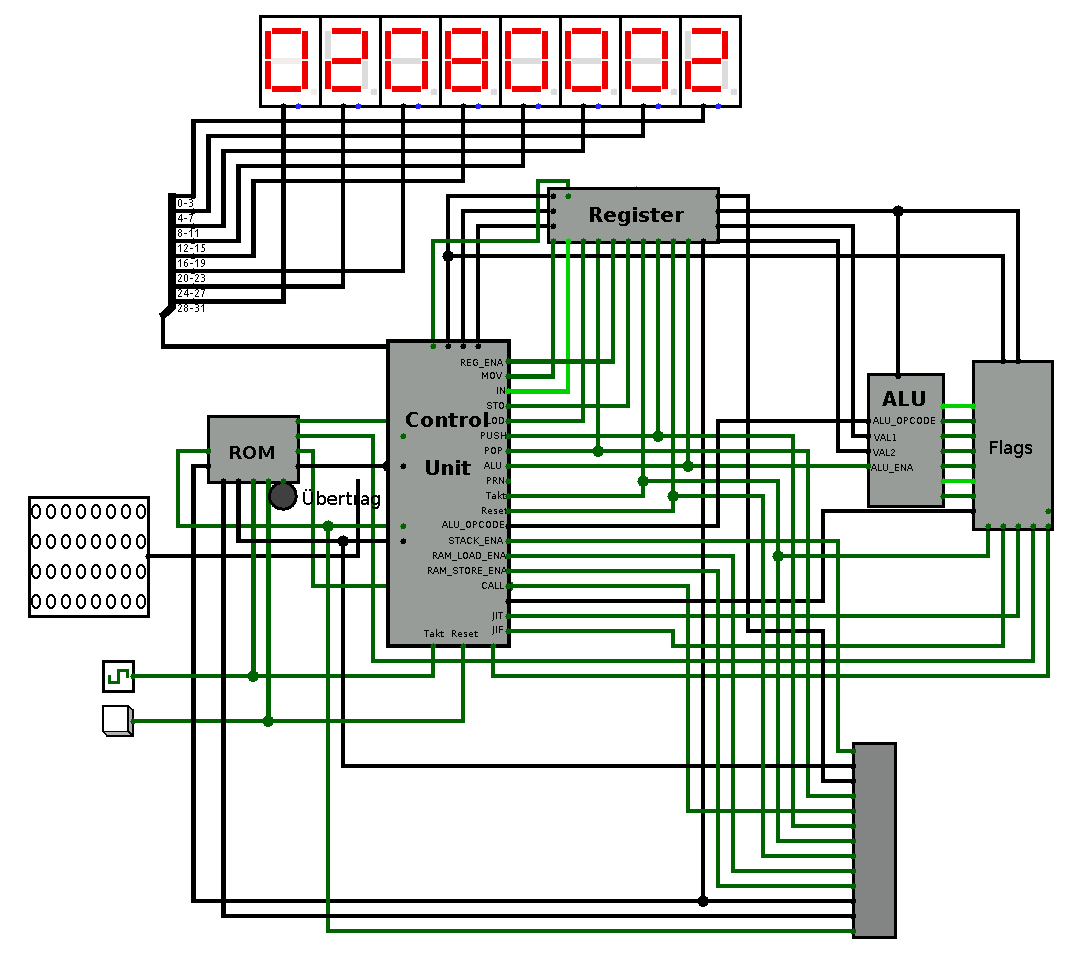
\includegraphics[scale=0.30]{cpu}
\caption{Darstellung des Prozessors}
\centering
\small Quelle: Eigene Darstellung
\label{fig:prozessor}
\end{figure}
\newpage



\subsection{Prozessor Komponenten}
Der Prozessor besteht aus fünf Hauptkomponenten:
\begin{itemize}
\item Control Unit - Steuerungseinheit (Abbildung \ref{fig:cu})
\item ALU - Arithmetisch Logische Einheit (Abbildung \ref{fig:alu})
\item Registersatz (Abbildung \ref{fig:register})
\item RAM/Stack (Abbildung \ref{fig:speicher})
\item ROM (Abbildung \ref{fig:rom})
\end{itemize}

\noindent Auf den folgenden Seiten werden Bilder der einzelnen Komponenten des Prozessors abgebildet.



\begin{figure}[!htbp]
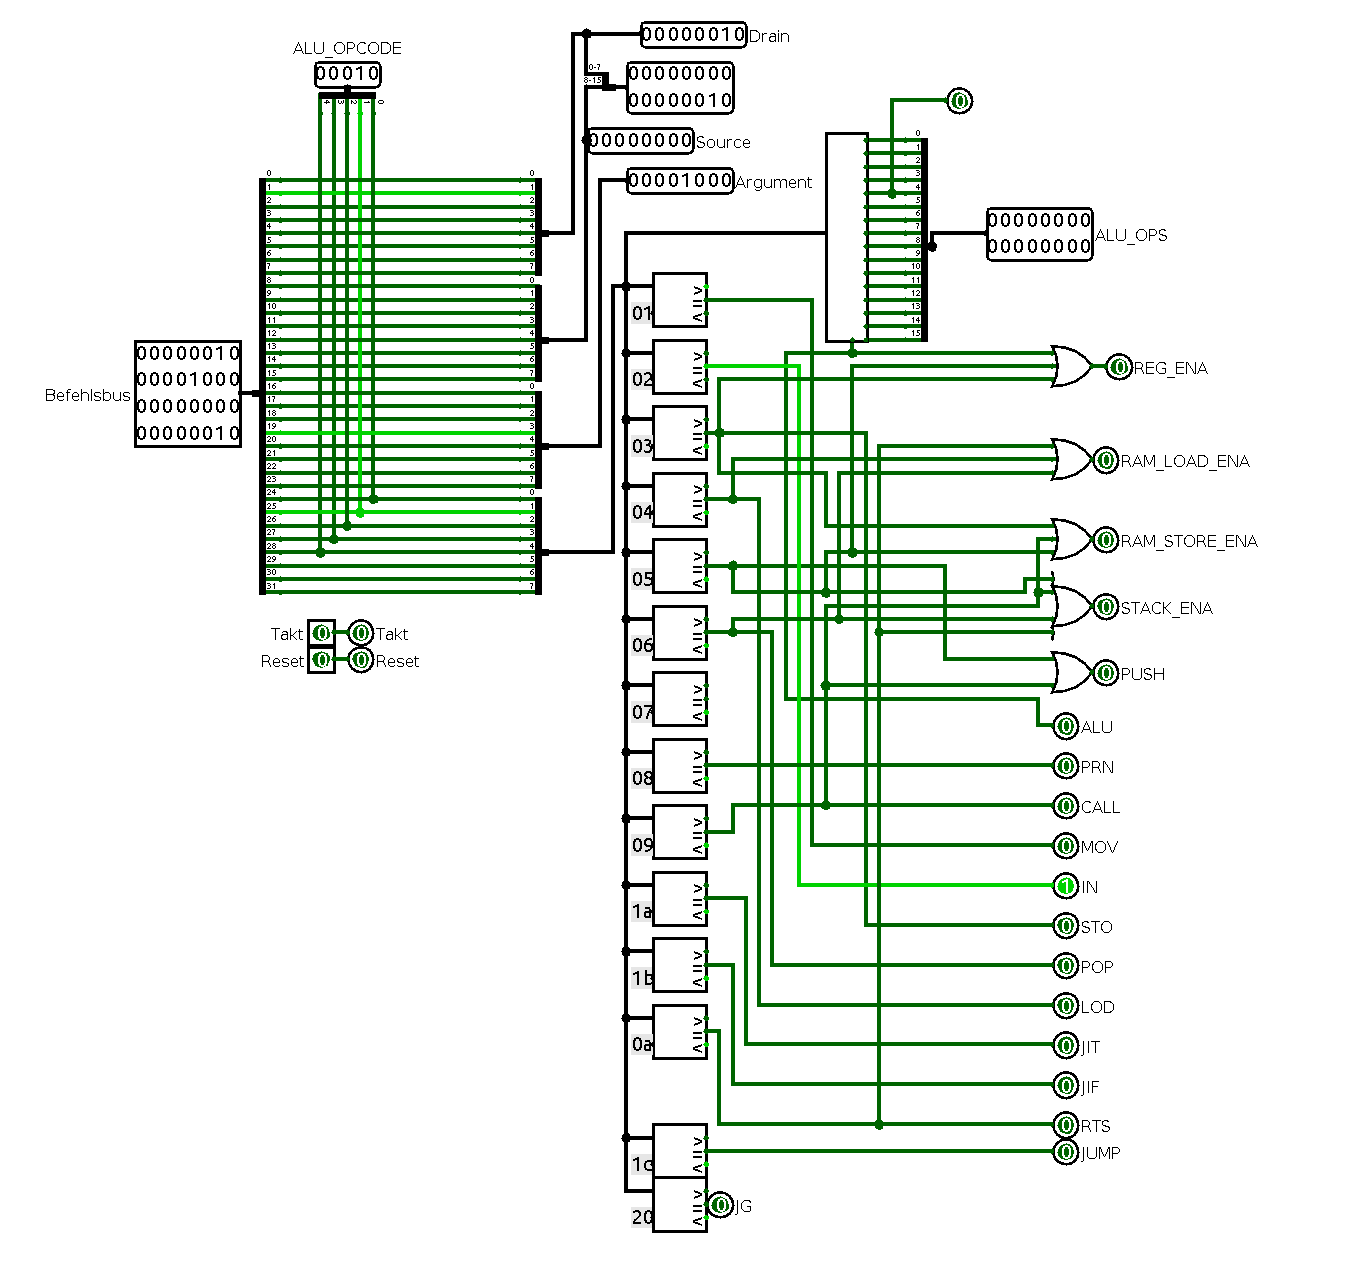
\includegraphics[scale=0.35]{cu}
\centering
\caption{Steuerwerk}
\centering
\small Quelle: Eigene Darstellung
\label{fig:cu}
\end{figure}
\newpage
\newpage


\begin{figure}[!htbp]
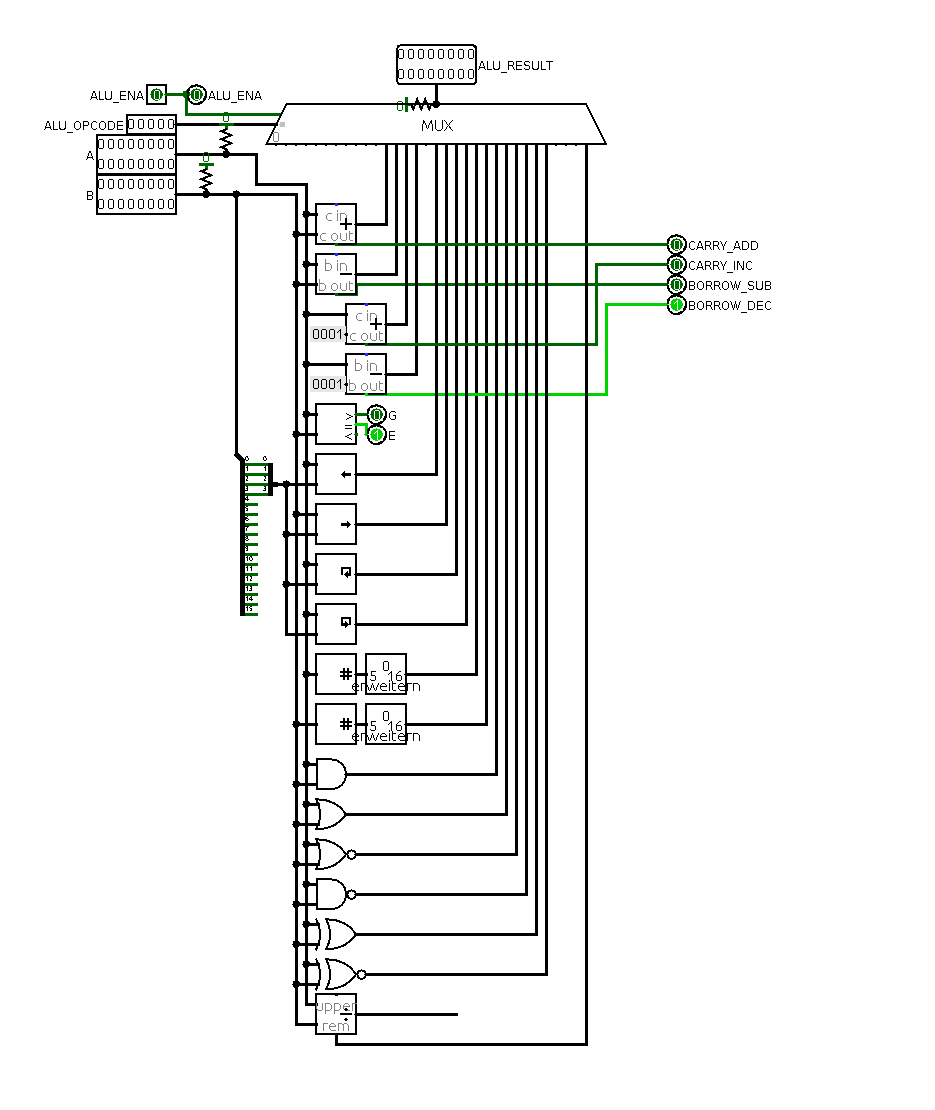
\includegraphics[scale=0.35]{alu}
\centering
\caption{Rechenwerk}
\centering
\small Quelle: Eigene Darstellung
\label{fig:alu}
\end{figure}

\newpage

\begin{figure}[!htbp]
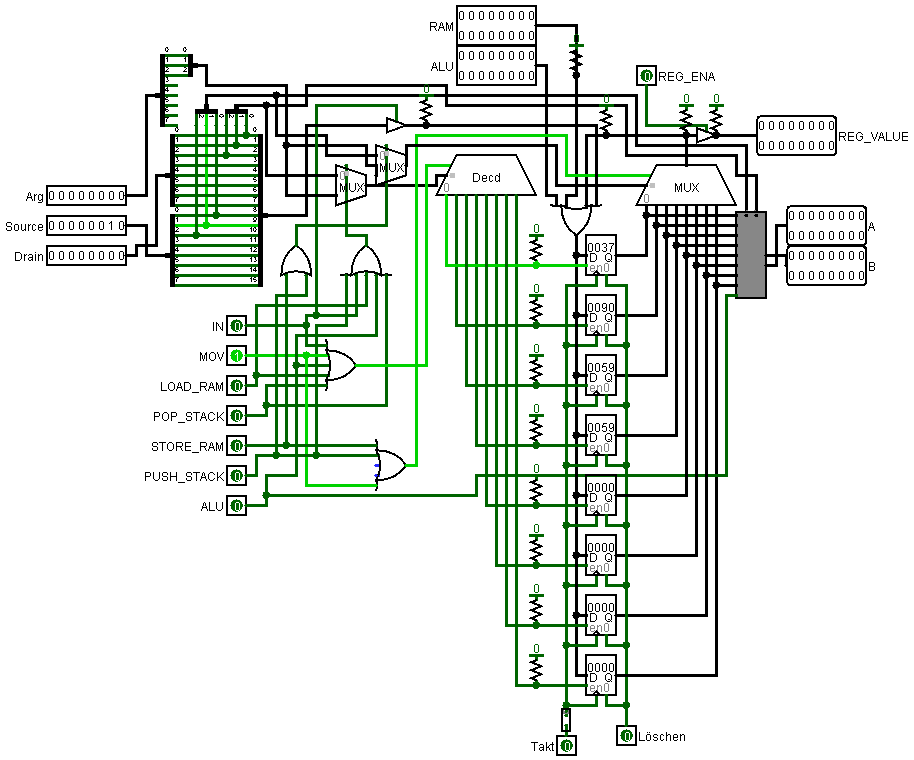
\includegraphics[scale=0.35]{register}
\centering
\caption{Registerwerk}
\centering
\small Quelle: Eigene Darstellung
\label{fig:register}
\end{figure}

\newpage

\begin{figure}[!hp]
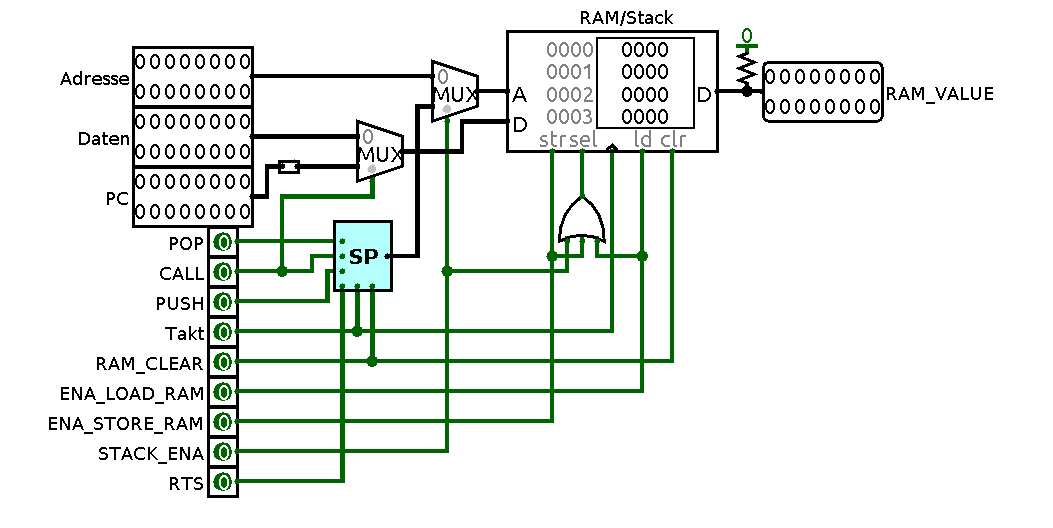
\includegraphics[scale=0.45]{ram}
\centering
\caption{Speicher}
\centering
\small Quelle: Eigene Darstellung
\label{fig:speicher}
\end{figure}

\begin{figure}[!hp]
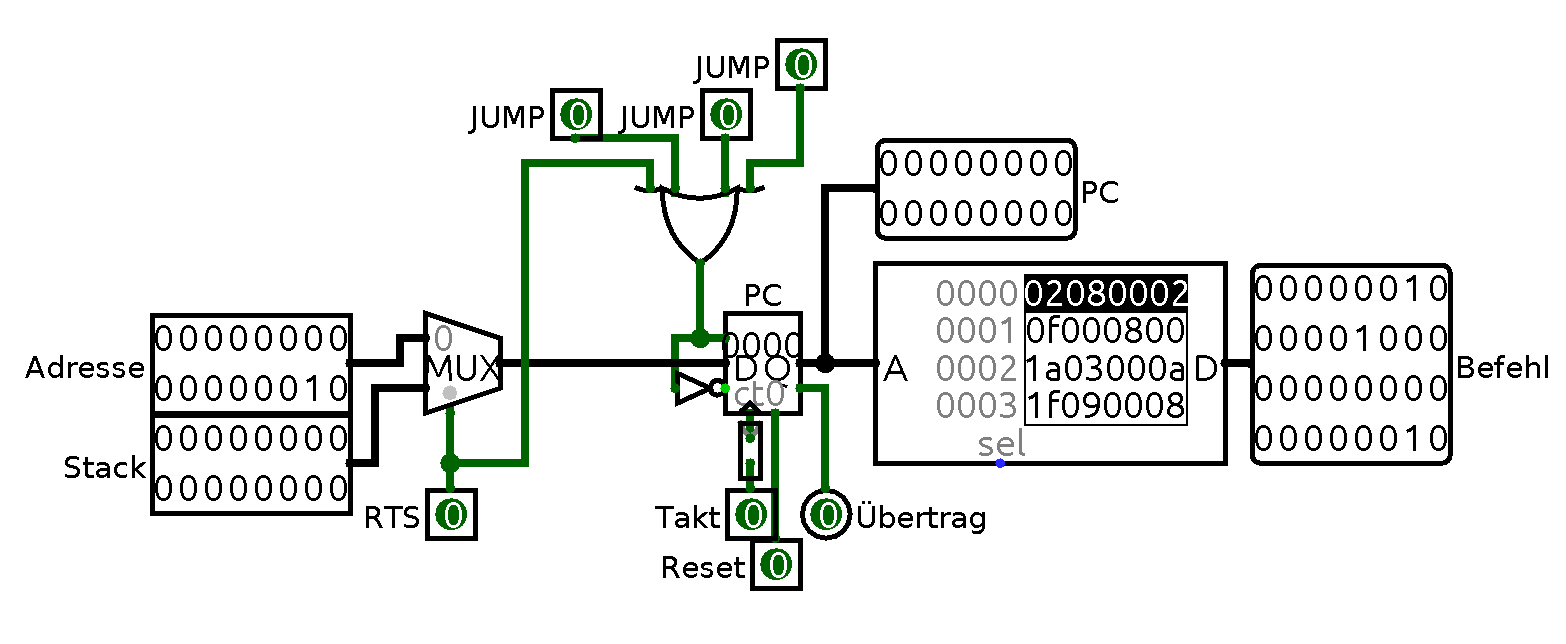
\includegraphics[scale=0.25]{rom}
\centering
\caption{ROM}
\centering
\small Quelle: Eigene Darstellung
\label{fig:rom}
\end{figure}
\newpage
\subsection{Entwicklung und Ausführung eines Programmes}
Um nun die Funktionalität der CPU zu zeigen wurde ein C++ Programm entwickelt, welches alle Primzahlen bis $2^{16} = 65536$ ausrechnet und die Anzahl der Primzahlen auf dem Terminal ausgibt. Dieses Programm wurde unter Ubuntu 17.10 mit dem Linuxkernel 4.13 kompiliert.

\begin{code}[!htb]
\begin{lstlisting}
bool checkIfPrime(unsigned int x){
	if(x<2) return false;
	unsigned int i=2;
	for(i;i<x;i++){
		if(x%i == 0){
			return false;
		}
	}
	return true;
}

int main(int argc, char const *argv[])
{
	int counter=0;
	for(unsigned int i=1;i<65536;i+=2){
		if(checkIfPrime(i)){
			counter++;
		}
	}
	std::cout << counter << std::endl; //Ausgabe 6541
	return 0;
}
\end{lstlisting}
\caption[C++ Code Primzahlenzählen]{C++ Code Primzahlenzählen}
\centering
\small Quelle: Eigene Darstellung
\label{code:prime}
\end{code}

\noindent Das in Quellcodeblock \ref{code:prime} gezeigte Programm zum Primzahlen zählen ist sehr ineffizient. Alleine die for-Schleife der CheckIfPrime-Funktion wird während des Ausführens 202.710.573 Schritte durchlaufen. Ziel ist nicht die optimale Laufzeit zu erreichen, sondern ein einfaches Programm auf der selbstgebauten CPU auszuführen.

\par\bigskip\noindent Um dieses Programm auf dem Prozessor ausführen zu können, muss es in der Assemblersprache der CPU neu geschrieben werden. Da Assembler eine sehr hardwarenahe Sprache ist, erleichtern wir uns die Entwicklung und betrachten den Assemblercode des C++ Programms, um die grobe Struktur sehen zu können, welche die CPU ausführt. Der Assemblercode kann mittels GDB betrachtet werden.
\newpage


\begin{code}
\begin{lstlisting}
   0x000000000040085e <+0>:	push   %rbp
   0x000000000040085f <+1>:	mov    %rsp,%rbp
   0x0000000000400862 <+4>:	sub    $0x20,%rsp
   0x0000000000400866 <+8>:	mov    %edi,-0x14(%rbp)
   0x0000000000400869 <+11>:	mov    %rsi,-0x20(%rbp)
   0x000000000040086d <+15>:	movl   $0x0,-0x8(%rbp)
   0x0000000000400874 <+22>:	movl   $0x1,-0x4(%rbp)
   0x000000000040087b <+29>:	cmpl   $0xffff,-0x4(%rbp)
   0x0000000000400882 <+36>:	ja     0x40089c <main+62>
   0x0000000000400884 <+38>:	mov    -0x4(%rbp),%eax
   0x0000000000400887 <+41>:	mov    %eax,%edi
   0x0000000000400889 <+43>:	callq  0x400816 <_Z12checkIfPrimej>
   0x000000000040088e <+48>:	test   %al,%al
   0x0000000000400890 <+50>:	je     0x400896 <main+56>
   0x0000000000400892 <+52>:	addl   $0x1,-0x8(%rbp)
   0x0000000000400896 <+56>:	addl   $0x2,-0x4(%rbp)
   0x000000000040089a <+60>:	jmp    0x40087b <main+29>
   0x000000000040089c <+62>:	mov    -0x8(%rbp),%eax
   0x000000000040089f <+65>:	mov    %eax,%esi
   0x00000000004008a1 <+67>:	mov    $0x601060,%edi
   0x00000000004008a6 <+72>:	callq  0x4006a0 <_ZNSolsEi@plt>
   0x00000000004008ab <+77>:	mov    $0x400700,%esi
   0x00000000004008b0 <+82>:	mov    %rax,%rdi
   0x00000000004008b3 <+85>:	callq  0x4006f0 <_ZNSolsEPFRSoS_E@plt>
   0x00000000004008b8 <+90>:	mov    $0x0,%eax
   0x00000000004008bd <+95>:	leaveq 
   0x00000000004008be <+96>:	retq   
\end{lstlisting}
\caption[Assemblercode der main Methode]{Assemblercode der main-Methode}
\centering
\small Quelle: Eigene Darstellung
\end{code}

\noindent In der Zeile main +15 wird die Variable counter mit 0 initialisiert und auf dem Stack an Offset 0x8 des Base Pointers platziert. 
Anschließend wird die Laufvariable i der for-Schleife in Zeile main+22 mit dem Wert 1 an Offset 0x4 des Base Pointers im Stack initialisiert.
\par\smallskip\noindent\textbf{Erster Durchlauf for-Schleife: } Zeile +29. Die Laufvariable i wird mit 0xffff (dezimal: 65536) verglichen. Anschließend wird mittels des Assembler-Befehls ja (jump if above) geprüft, welche Flag der vorherige Compare Befehl gesetzt hat. Wenn im Flagregister das greater Bit gesetzt wurde, springt das Programm an die Adresse $0x40089c$ (main+62), also aus for-Schleife raus, da die Schleifenbedingung $(i<65536)$ nicht mehr erfüllt ist. Wenn kein Sprung auftritt, läuft das Programm weiter und ruft an Stelle main+43 die Funktion checkIfPrime auf. Diese Funktion erwartet allerdings einen Übergabeparameter; dieser wird in Register \$edi (main+41)abgelegt. 
Der Rückgabewert der Funktion steht daraufhin, wenn die Funktion durchlaufen und beendet wurde, in Register al. Da checkIfPrime den Rückgabetyp boolean besitzt, steht in Register al entweder eine 0, wenn es keine Primzahl war oder 1, wenn es eine Primzahl war, die übergeben wurde. Der Befehl test an Stelle main+48 führt ein bitweise logisches UND zwischen al und al aus. Hier prüft der Prozessor, ob das Ergebnis ungleich null war und setzt das ZF-Bit (Zero Flag). Wenn das Flag-Bit nicht gesetzt wurde, wird das Programm ganz normal weitergeführt. Die counter Variable wird inkrementiert (main+52) und die Laufvariable i wird um zwei erhöht (main+56), daraufhin wird an Stelle main+29 gesprungen und der nächste Schleifendurchgang beginnt.

\begin{code}[!htb]
\begin{lstlisting}
Dump of assembler code for function _Z12checkIfPrimej:
   0x0000000000400816 <+0>:	push   %rbp
   0x0000000000400817 <+1>:	mov    %rsp,%rbp
   0x000000000040081a <+4>:	mov    %edi,-0x14(%rbp)
   0x000000000040081d <+7>:	cmpl   $0x1,-0x14(%rbp)
   0x0000000000400821 <+11>:	ja     0x40082a <_Z12checkIfPrimej+20>
   0x0000000000400823 <+13>:	mov    $0x0,%eax
   0x0000000000400828 <+18>:	jmp    0x40085c <_Z12checkIfPrimej+70>
   0x000000000040082a <+20>:	movl   $0x2,-0x4(%rbp)
   0x0000000000400831 <+27>:	mov    -0x4(%rbp),%eax
   0x0000000000400834 <+30>:	cmp    -0x14(%rbp),%eax
   0x0000000000400837 <+33>:	jae    0x400857 <_Z12checkIfPrimej+65>
   0x0000000000400839 <+35>:	mov    -0x14(%rbp),%eax
   0x000000000040083c <+38>:	mov    $0x0,%edx
   0x0000000000400841 <+43>:	divl   -0x4(%rbp)
   0x0000000000400844 <+46>:	mov    %edx,%eax
   0x0000000000400846 <+48>:	test   %eax,%eax
   0x0000000000400848 <+50>:	jne    0x400851 <_Z12checkIfPrimej+59>
   0x000000000040084a <+52>:	mov    $0x0,%eax
   0x000000000040084f <+57>:	jmp    0x40085c <_Z12checkIfPrimej+70>
   0x0000000000400851 <+59>:	addl   $0x1,-0x4(%rbp)
   0x0000000000400855 <+63>:	jmp    0x400831 <_Z12checkIfPrimej+27>
   0x0000000000400857 <+65>:	mov    $0x1,%eax
   0x000000000040085c <+70>:	pop    %rbp
   0x000000000040085d <+71>:	retq   
End of assembler dump.

\end{lstlisting}
\caption[Assemblercode der checkIfPrime Methode]{Assemblercode der checkIfPrime-Methode}
\centering
\small Quelle: Eigene Darstellung
\end{code}
%Intel Dokumentation zitieren Code Listing 3 URL-
%https://software.intel.com/sites/default/files/managed/a4/60/325383-sdm-vol-2abcd.pdf
\noindent Das Code Listing 3 zeigt den Assemblercode der Funktion checkIfPrime. In Zeile 4 wird der Übergabeparameter, welcher sich in Register edi befindet, auf den Stack verschoben. Daraufhin wird mit dem Befehl cmpl dieser Übergabeparameter mit dem Wert 1 verglichen. Dafür werden die beiden Werte subtrahiert und das Ergebnis ausgewertet. Bei dieser Auswertung setzt die CPU automatisch die Flags für die Subtraktion. Wenn Beispielweise eine -2 übergeben wird und vom Befehl compl mit dem Wert 1 verglichen werden soll, so wird die ALU -2-1=-3 rechnen und dabei die Sign Flag(SF) setzen, da das Ergebnis negativ ist. Der nächste Befehl ist jg (Jump if greater), dieser Sprung wird laut Intel-Architektur-Dokumentation nur ausgeführt, wenn die beiden Flags ZF und SF nicht gesetzt, also null sind. Diese sind null, wenn das Ergebnis zum einen nicht negativ (SF) und nicht null (ZF) ist. \newline Kurz gesagt: Die beiden Zeilen 7 und 11 stellen sicher, dass der Übergabeparameter größer als 1 ist. Im C++ Programm entspricht das der ersten Zeile der Funktion. Sollte eine der beiden Flags ZF bzw. SF nicht gesetzt sein, wird nicht gesprungen und in Zeile 13 eine 0 in das Rückgaberegister geschrieben. Daraufhin wird zum Ende der Funktion gesprungen und die Funktion ist beendet. Wenn der Sprung in Zeile 11 ausgeführt wird, dann springt das Programm zu Zeile 20 in der die Laufvariable i  mit dem Wert 2 initialisiert wird. Die Zeilen 27 bis 30 sind analog zu Codelisting 2 die Prüfung der Laufvariable in der for-Schleife, ob die Abbruchbedinggung bereits erfüllt ist \cite{c}. In der Schleife werden die Zeilen 35 bis 59 ausgeführt. Der Befehl idvl führt eine Division aus, wobei der Rest in Register EDX gespeichert wird. Nachdem EDX in EAX verschoben wurde, wird mittels des Befehls test EAX,EAX (Zeile 48) geprüft, ob das Register null ist, also auch der Rest der Division null ist. Sollte dem so sein, so springt das Programm ans Ende und schreibt eine 0 in Übergaberegister EAX\cite[S.202]{technischeInformatik2}.
\newpage

\section{Schlusswort}
Prozessoren haben wie keine andere Technik die Entwicklung der Informatik beeinflusst. Sie sind die Grundlage jedes Computers, ganz gleich, ob sie in einem Mobiltelefon oder einem Server eingesetzt werden. In den letzten 20 Jahren wurde die Leistungsfähigkeit der Prozessoren immer weiter gesteigert. Zuerst durch immer höhere Taktraten, später dann durch mehrere CPU-Kerne und Veränderungen an der Architektur. Goorden Moore, einer der Gründer von Intel, hat 1965 das Moorsche Gesetz in einem Artikel beschrieben. Danach verdoppelt sich die Anzahl an Transistoren auf den Chips alle 18 Monate. Diese Entwicklung kann bis heute nachverfolgt werden. Allerdings kann dieser Trend nicht immer so weitergehen. 

\par\bigskip\noindent Die Forschung an Quantencomputern zeigt neuerdings immer größere Erfolge. Die zukünftige Entwicklung der Prozessoren bleibt also spannend. 
\newpage
\pagestyle{empty}

\addcontentsline{toc}{section}{Abbildungsverzeichnis}
\listoffigures
\newpage
\addcontentsline{toc}{section}{Tabellenverzeichnis}
\listoftables
\newpage
\addcontentsline{toc}{section}{Quellcodeverzeichnis}
\listofcodes
\newpage
\addcontentsline{toc}{section}{Literaturverzeichnis}
\bibliography{Referenzen}

\newpage
\section*{Eidesstattliche Erklärung}

Hiermit erkläre ich, dass ich die vorliegende Seminararbeit
mit dem Titel „Aufbau und Funktionsweise eines Prozessors“ selbständig verfasst habe, dass ich sie
zuvor an keiner anderen Hochschule und in keinem
anderen Studiengang als Prüfungsleistung eingereicht
habe und dass ich keine anderen als die angegebenen
Quellen und Hilfsmittel benutzt habe. Alle Stellen der
Arbeit, die wörtlich oder sinngemäß aus Veröffentlichungen
oder aus anderweitigen fremden Äußerungen entnommen
wurden, sind als solche kenntlich gemacht.\bigskip

\noindent
Hof, den \today

\vspace*{2cm}

\begin{tabular}{@{}l@{}}\hline
\rule{0pt}{2ex}
Marco Vogel
\end{tabular}

\end{document}



















